%%%%%%%%%%%%%%%%%%%%%%%%%%%%%%%%%%%%%%%%%
% Masters/Doctoral Thesis 
% LaTeX Template
% Version 1.43 (17/5/14)
%
% This template has been downloaded from:
% http://www.LaTeXTemplates.com
%
% Original authors:
% Steven Gunn 
% http://users.ecs.soton.ac.uk/srg/softwaretools/document/templates/
% and
% Sunil Patel
% http://www.sunilpatel.co.uk/thesis-template/
%
% License:
% CC BY-NC-SA 3.0 (http://creativecommons.org/licenses/by-nc-sa/3.0/)
%
% Note:
% Make sure to edit document variables in the Thesis.cls file
%
%%%%%%%%%%%%%%%%%%%%%%%%%%%%%%%%%%%%%%%%%

%----------------------------------------------------------------------------------------
%	PACKAGES AND OTHER DOCUMENT CONFIGURATIONS
%----------------------------------------------------------------------------------------

\documentclass[11pt, oneside]{Thesis} % The default font size and one-sided printing (no margin offsets)

\graphicspath{{Pictures/}} % Specifies the directory where pictures are stored

\usepackage[square, numbers, comma, sort&compress]{natbib} % Use the natbib reference package - read up on this to edit the reference style; if you want text (e.g. Smith et al., 2012) for the in-text references (instead of numbers), remove 'numbers' 


\usepackage{subfigure}
\usepackage{amsmath}
\usepackage{multirow}
\usepackage{algorithmicx}
\usepackage[ruled]{algorithm}
\usepackage{algpseudocode}
\usepackage{color}
\usepackage{algpascal}
\usepackage{algc}


\hypersetup{urlcolor=blue, colorlinks=true} % Colors hyperlinks in blue - change to black if annoying
\title{\ttitle} % Defines the thesis title - don't touch this

\begin{document}

\frontmatter % Use roman page numbering style (i, ii, iii, iv...) for the pre-content pages

\setstretch{1.3} % Line spacing of 1.3

% Define the page headers using the FancyHdr package and set up for one-sided printing
\fancyhead{} % Clears all page headers and footers
\rhead{\thepage} % Sets the right side header to show the page number
\lhead{} % Clears the left side page header

\pagestyle{fancy} % Finally, use the "fancy" page style to implement the FancyHdr headers

\newcommand{\HRule}{\rule{\linewidth}{0.5mm}} % New command to make the lines in the title page

% PDF meta-data
\hypersetup{pdftitle={\ttitle}}
\hypersetup{pdfsubject=\subjectname}
\hypersetup{pdfauthor=\authornames}
\hypersetup{pdfkeywords=\keywordnames}

%----------------------------------------------------------------------------------------
%	TITLE PAGE
%----------------------------------------------------------------------------------------

\begin{titlepage}
\begin{center}

\textsc{\LARGE \univname}\\[1.5cm] % University name
\textsc{\Large Doctoral Thesis}\\[0.5cm] % Thesis type

\HRule \\[0.4cm] % Horizontal line
{\huge \bfseries \ttitle}\\[0.4cm] % Thesis title
\HRule \\[1.5cm] % Horizontal line
 
\begin{minipage}{0.4\textwidth}
\begin{flushleft} \large
\emph{Author:}\\
\href{http://www.johnsmith.com}{\authornames} % Author name - remove the \href bracket to remove the link
\end{flushleft}
\end{minipage}
\begin{minipage}{0.4\textwidth}
\begin{flushright} \large
\emph{Supervisor:} \\
\href{http://www.jamessmith.com}{\supname} % Supervisor name - remove the \href bracket to remove the link  
\end{flushright}
\end{minipage}\\[3cm]
 
\large \textit{A thesis submitted in fulfilment of the requirements\\ for the degree of \degreename}\\[0.3cm] % University requirement text
\textit{in the}\\[0.4cm]
\groupname\\\deptname\\[2cm] % Research group name and department name
 
{\large \today}\\[4cm] % Date
%\includegraphics{Logo} % University/department logo - uncomment to place it
 
\vfill
\end{center}

\end{titlepage}

%----------------------------------------------------------------------------------------
%	DECLARATION PAGE
%	Your institution may give you a different text to place here
%----------------------------------------------------------------------------------------

\Declaration{

\addtocontents{toc}{\vspace{1em}} % Add a gap in the Contents, for aesthetics

I, \authornames, declare that this thesis titled, '\ttitle' and the work presented in it are my own. I confirm that:

\begin{itemize} 
\item[\tiny{$\blacksquare$}] This work was done wholly or mainly while in candidature for a research degree at this University.
\item[\tiny{$\blacksquare$}] Where any part of this thesis has previously been submitted for a degree or any other qualification at this University or any other institution, this has been clearly stated.
\item[\tiny{$\blacksquare$}] Where I have consulted the published work of others, this is always clearly attributed.
\item[\tiny{$\blacksquare$}] Where I have quoted from the work of others, the source is always given. With the exception of such quotations, this thesis is entirely my own work.
\item[\tiny{$\blacksquare$}] I have acknowledged all main sources of help.
\item[\tiny{$\blacksquare$}] Where the thesis is based on work done by myself jointly with others, I have made clear exactly what was done by others and what I have contributed myself.\\
\end{itemize}
 
Signed:\\
\rule[1em]{25em}{0.5pt} % This prints a line for the signature
 
Date:\\
\rule[1em]{25em}{0.5pt} % This prints a line to write the date
}

\clearpage % Start a new page

%----------------------------------------------------------------------------------------
%	QUOTATION PAGE
%----------------------------------------------------------------------------------------

\pagestyle{empty} % No headers or footers for the following pages

\null\vfill % Add some space to move the quote down the page a bit

\textit{``Thanks to my solid academic training, today I can write hundreds of words on virtually any topic without possessing a shred of information, which is how I got a good job in journalism."}

\begin{flushright}
Dave Barry
\end{flushright}

\vfill\vfill\vfill\vfill\vfill\vfill\null % Add some space at the bottom to position the quote just right

\clearpage % Start a new page

%----------------------------------------------------------------------------------------
%	ABSTRACT PAGE
%----------------------------------------------------------------------------------------

\addtotoc{Abstract} % Add the "Abstract" page entry to the Contents

\abstract{\addtocontents{toc}{\vspace{1em}} % Add a gap in the Contents, for aesthetics

The Thesis Abstract is written here (and usually kept to just this page). The page is kept centered vertically so can expand into the blank space above the title too\ldots
}

\clearpage % Start a new page

%----------------------------------------------------------------------------------------
%	ACKNOWLEDGEMENTS
%----------------------------------------------------------------------------------------

\setstretch{1.3} % Reset the line-spacing to 1.3 for body text (if it has changed)

\acknowledgements{\addtocontents{toc}{\vspace{1em}} % Add a gap in the Contents, for aesthetics

The acknowledgements and the people to thank go here, don't forget to include your project advisor\ldots
}
\clearpage % Start a new page

%----------------------------------------------------------------------------------------
%	LIST OF CONTENTS/FIGURES/TABLES PAGES
%----------------------------------------------------------------------------------------

\pagestyle{fancy} % The page style headers have been "empty" all this time, now use the "fancy" headers as defined before to bring them back

\lhead{\emph{Contents}} % Set the left side page header to "Contents"
\tableofcontents % Write out the Table of Contents

\lhead{\emph{List of Figures}} % Set the left side page header to "List of Figures"
\listoffigures % Write out the List of Figures

\lhead{\emph{List of Tables}} % Set the left side page header to "List of Tables"
\listoftables % Write out the List of Tables

%----------------------------------------------------------------------------------------
%	ABBREVIATIONS
%----------------------------------------------------------------------------------------

\clearpage % Start a new page

\setstretch{1.5} % Set the line spacing to 1.5, this makes the following tables easier to read

\lhead{\emph{Abbreviations}} % Set the left side page header to "Abbreviations"
\listofsymbols{ll} % Include a list of Abbreviations (a table of two columns)
{
\textbf{LAH} & \textbf{L}ist \textbf{A}bbreviations \textbf{H}ere \\
%\textbf{Acronym} & \textbf{W}hat (it) \textbf{S}tands \textbf{F}or \\
}

%----------------------------------------------------------------------------------------
%	PHYSICAL CONSTANTS/OTHER DEFINITIONS
%----------------------------------------------------------------------------------------

\clearpage % Start a new page

\lhead{\emph{Physical Constants}} % Set the left side page header to "Physical Constants"

\listofconstants{lrcl} % Include a list of Physical Constants (a four column table)
{
Speed of Light & $c$ & $=$ & $2.997\ 924\ 58\times10^{8}\ \mbox{ms}^{-\mbox{s}}$ (exact)\\
% Constant Name & Symbol & = & Constant Value (with units) \\
}

%----------------------------------------------------------------------------------------
%	SYMBOLS
%----------------------------------------------------------------------------------------

\clearpage % Start a new page

\lhead{\emph{Symbols}} % Set the left side page header to "Symbols"

\listofnomenclature{lll} % Include a list of Symbols (a three column table)
{
$a$ & distance & m \\
$P$ & power & W (Js$^{-1}$) \\
% Symbol & Name & Unit \\

& & \\ % Gap to separate the Roman symbols from the Greek

$\omega$ & angular frequency & rads$^{-1}$ \\
% Symbol & Name & Unit \\
}

%----------------------------------------------------------------------------------------
%	DEDICATION
%----------------------------------------------------------------------------------------

\setstretch{1.3} % Return the line spacing back to 1.3

\pagestyle{empty} % Page style needs to be empty for this page

\dedicatory{For/Dedicated to/To my\ldots} % Dedication text

\addtocontents{toc}{\vspace{2em}} % Add a gap in the Contents, for aesthetics

%----------------------------------------------------------------------------------------
%	THESIS CONTENT - CHAPTERS
%----------------------------------------------------------------------------------------

\mainmatter % Begin numeric (1,2,3...) page numbering

\pagestyle{fancy} % Return the page headers back to the "fancy" style

% Include the chapters of the thesis as separate files from the Chapters folder
% Uncomment the lines as you write the chapters

% Chapter 1

\chapter{Introduction} % Main chapter title

\label{intro} % For referencing the chapter elsewhere, use \ref{Chapter1} 

\lhead{Introduction \emph{Wireless Sensor Network}} % This is for the header on each page - perhaps a shortened title

%----------------------------------------------------------------------------------------

\section{Wireless Sensor Networks}

Write about wsn, recent advances, growth, applications, briefly.
Write about internals of wsn : hardware, software.

\subsection{Application}

Write about applications : mobile and otherwise

\subsection{Challenges}

Challenges in static WSN and WSN in general

\section{Mobile Wireless Sensor network}

Write about internals of MWSN : hardware, software.

\subsection{Application}

Write about applications : mobile 

\subsection{Challenges}

Challenges in MWSN

\section{Cross Layer Architecture}
\subsection{Overview}
\subsection{Need for Cross Layer Architecture}

% Chapter 1

\chapter{Background} % Main chapter title

\label{bg} % For referencing the chapter elsewhere, use \ref{Chapter1} 

\lhead{Background} % This is for the header on each page - perhaps a shortened title

%----------------------------------------------------------------------------------------

\section{Challenges}

Need for time synchronization and mobility estimation.

\section{Mobility-aware MAC protocols}

There are a number of MAC protocols available for WSN that support mobility. Each of these protocols is specially designed to support a specific type of mobility pattern encountered in a specific real life WSN scenario. In the following subsections, we briefly discuss the existing Mobility-aware MAC protocols for WSN.\\

\subsection{Challenges}
What parameters should be considered? Mobile vs Static

\subsection{Existing Techniques}


\begin{figure}[h]{} 
  \begin{center}
		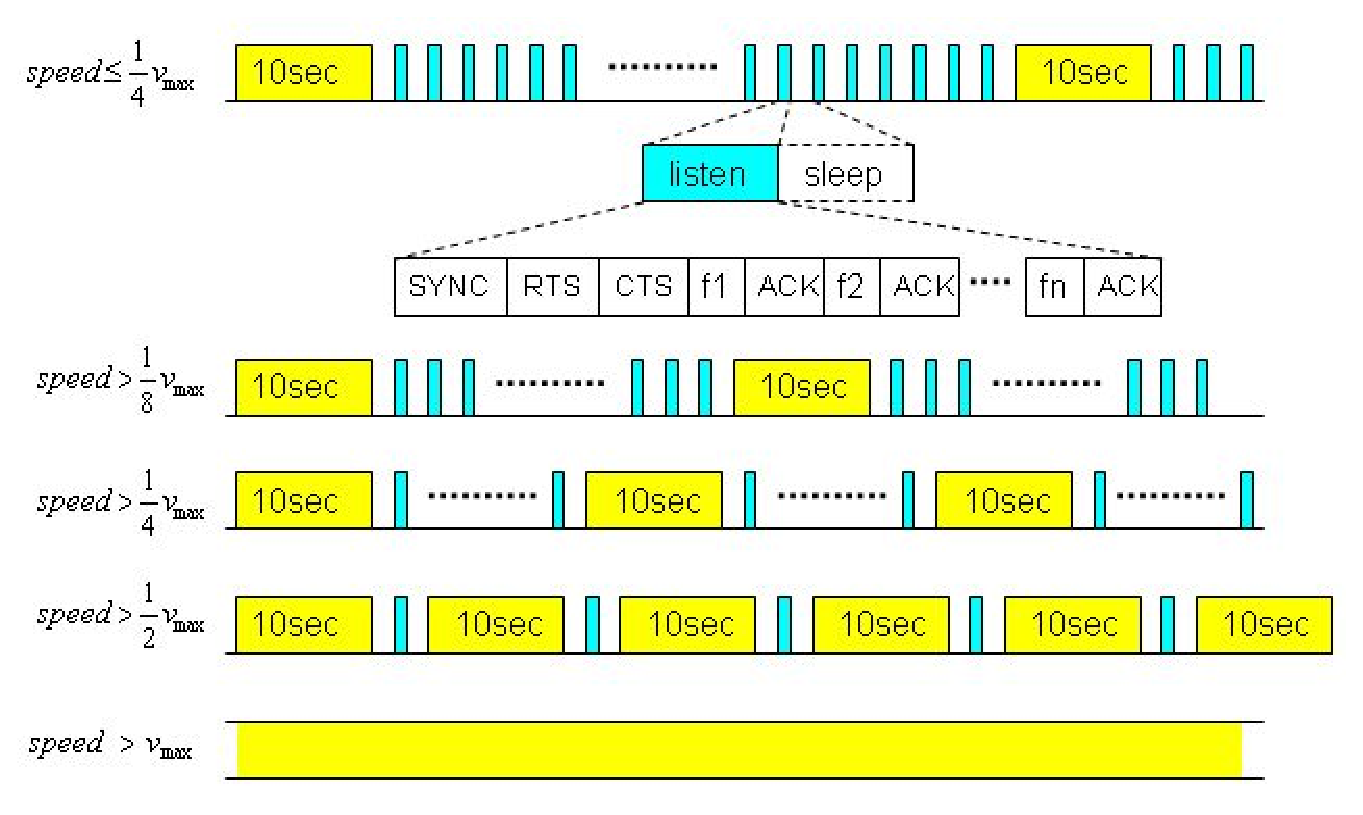
\includegraphics[scale=0.3, natwidth=0.38\textwidth]{msmac_timing}
		\caption{MS-MAC Timing Diagram}
	\label{fig:msmac-timing}
  \end{center}
\end{figure}



\subsubsection{MS-MAC}
%--- A para on current MAC protocol available. Classify them as Schedule based and contention based protocol. Why Schedule based protocol are better? Advantage of TDMA based protocols. --- \\ \\
 MS-MAC \cite{ms-mac} is a derivative of SMAC \cite{smac}, extended to support mobility. SMAC makes use of duty cycling to increase the sleep time of each node. This sleep/wake schedule is not global. In fact, SMAC organizes the network into virtual clusters, where nodes which possess a common schedule are grouped together as a cluster. The mobility information of each nodes is observed by the other nodes in the cluster. Based on the variation in the RSSI value of a mobile node, inter-cluster mobility of the node is detected by the cluster members. The cluster members then, form an active zone for a period of time, during with they adjust their synchronization frequency to support the mobile node in reaching the new cluster without losing connection to all its neighbours. \\\\

\begin{figure}[h]{} 
  \begin{center}
		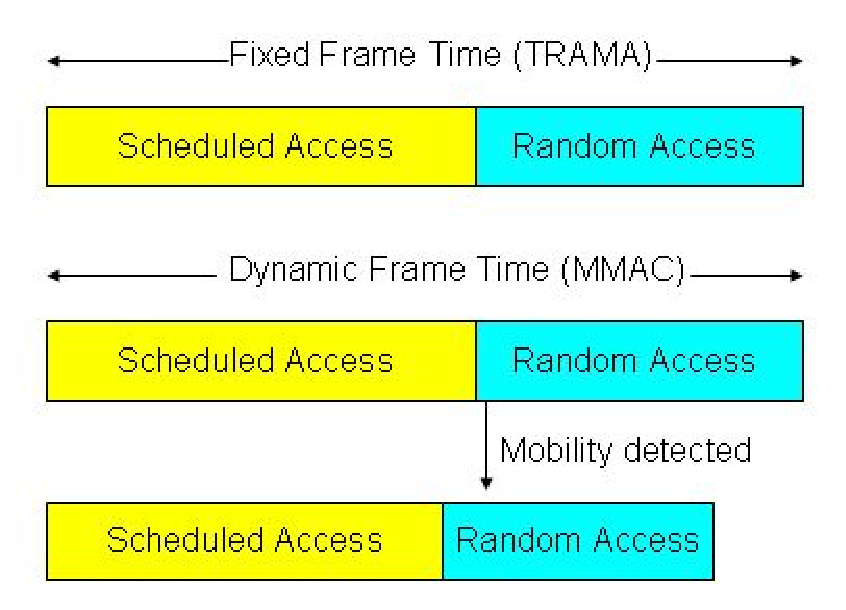
\includegraphics[scale=0.3, natwidth=0.38\textwidth]{mmac_timing}
		\caption{M-MAC Timing Diagram}
	\label{fig:mmac-timing}
  \end{center}
\end{figure}


\subsubsection{M-MAC}
M-MAC \cite{m-mac} is a scheduling based MAC protocol that employs a flexible frame time to adapt to mobility. Each round is divided into \emph{k} frames. During each frame, every node predicts its own location estimate for the next frame. This estimate is transmitted to the cluster head. The cluster head gathers the location information from each node, aggregates it and broadcasts it during the last slot of the current frame. This information provides the nodes in the cluster the knowledge of the mobility states of the cluster members, based on which a node chooses one of its neighbours to relay the data packets.

\begin{figure}[h]{} 
  \begin{center}
		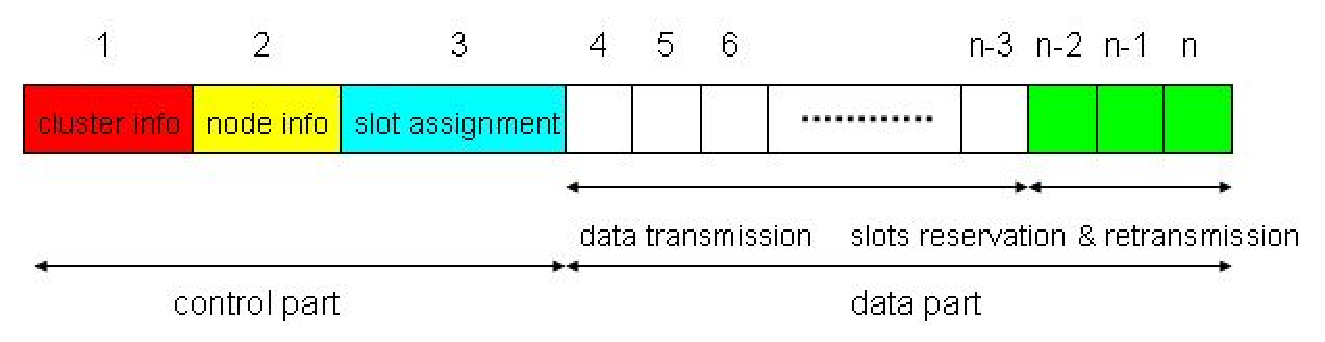
\includegraphics[scale=0.3, natwidth=0.38\textwidth]{mtdma_timing}
		\caption{M-TDMA: Timing Diagram}
	\label{fig:mtdma-timing}
  \end{center}
\end{figure}


\subsubsection{M-TDMA}
M-TDMA \cite{m-tdma} partitions the network into non-overlapping clusters based on FLOC algorithm\cite{floc}. Each cluster maintains a frame where a unique slot is provided for each cluster member. The slots are divided into control, data and reserved slots. The reserved slots are reserved for join requests from new nodes entering the cluster and message retransmissions. The control slots are divided to accomodate cluster information, node information and slot assignment. 

\begin{figure}[h]{} 
  \begin{center}
		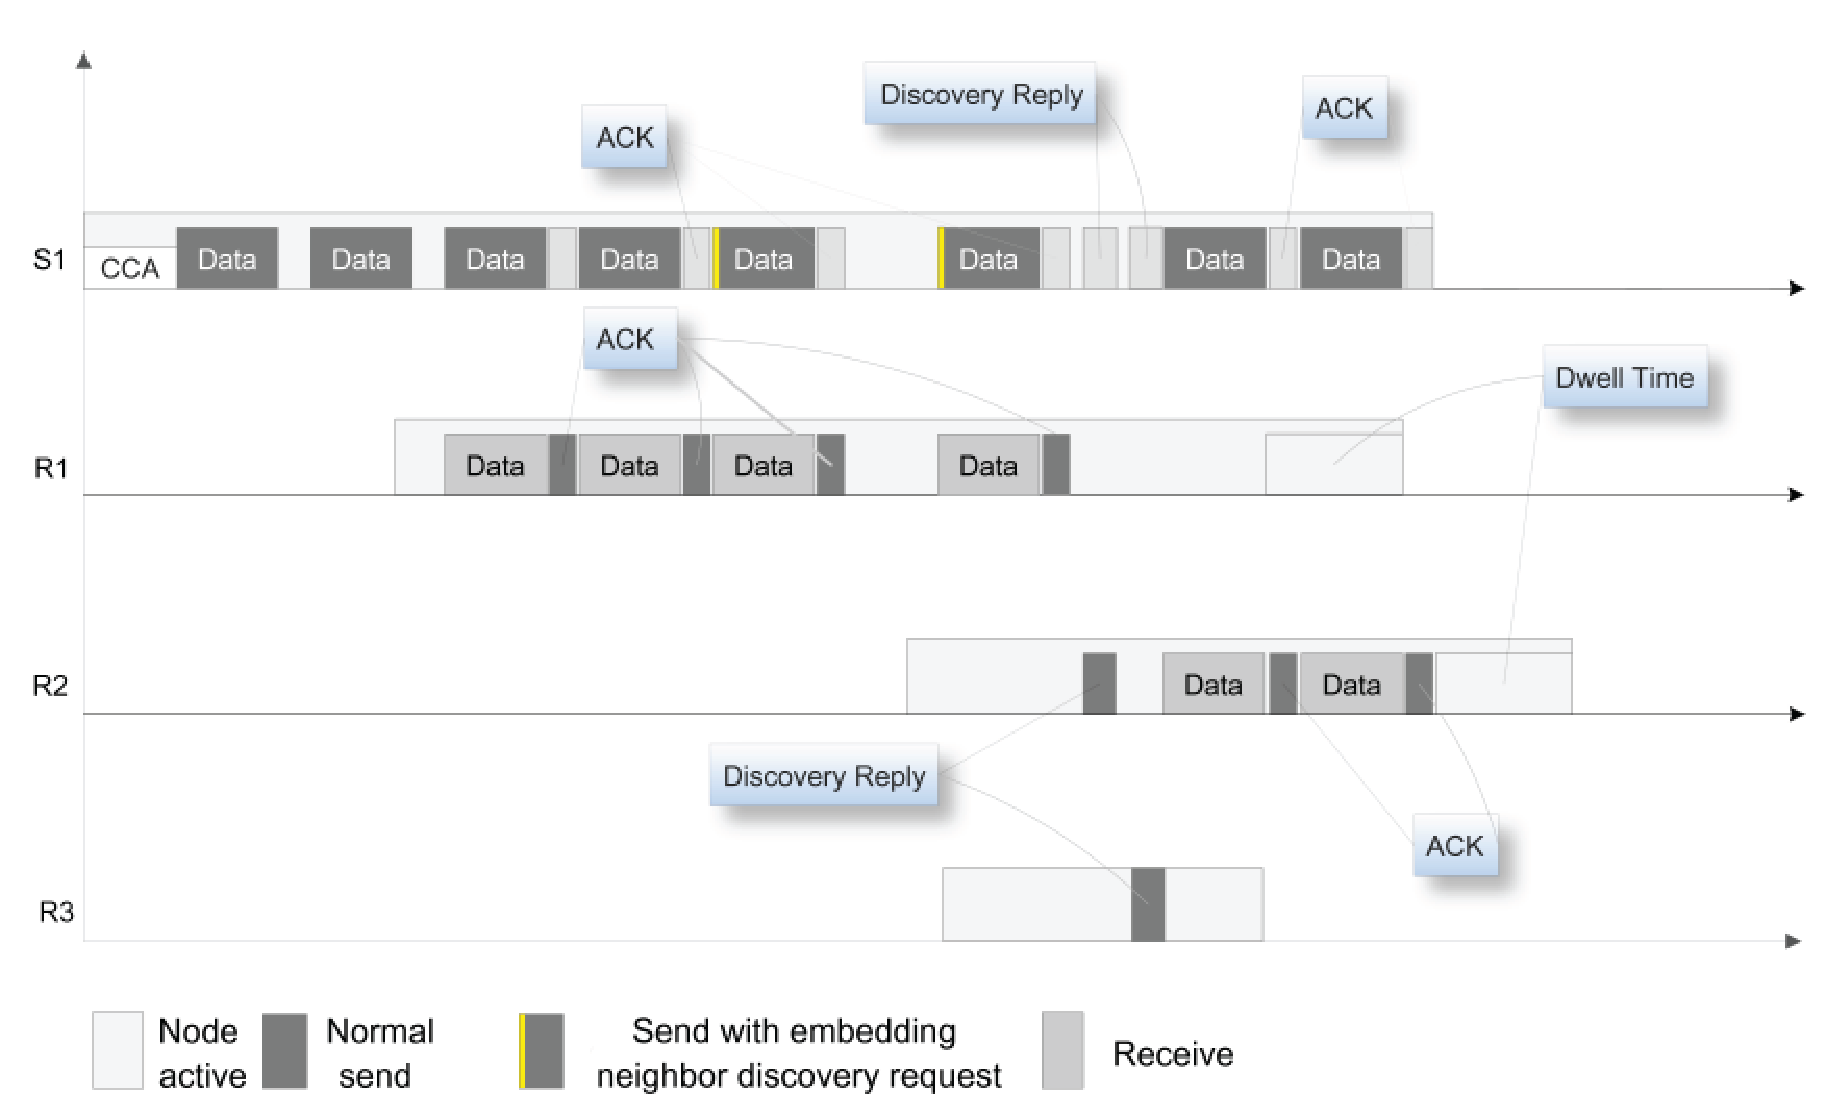
\includegraphics[scale=0.3, natwidth=0.38\textwidth]{mamac_timing}
		\caption{MA-MAC : Timing Diagram}
	\label{fig:mamac-timing}
  \end{center}
\end{figure}


\subsubsection{MA-MAC}
MA-MAC \cite{ma-mac} is a contention based protocol that primarily focusses on reliability of data transfer through seamless handover by adopting two distance thresholds. A sender \emph{$S_1$} initiates communication by transmitting a preamble packet to a receiver \emph{$R_1$}. When the receiver replies with an ACK message, the sender continues sending data packets. Over a period of time, the sender accumulates enough history RSSI values from the ACK packets sent by \emph{$R_1$}. At this point of time, it estimates its distance to the receiver. \emph{$S_1$} monitor this distance to see if it exceeds the distance threshold. When it exceeds the first threshold, \emph{$S_1$} starts embedding handover requests with the data packets, which it is broadcasting now. When another node \emph{$R_2$} receives this handover request, it replies with a handover reply. Now \emph{$S_1$} starts unicasting the data packets to \emph{$R_2$} instead of \emph{$R_1$}.  
 
\begin{figure}[h]{} 
  \begin{center}
		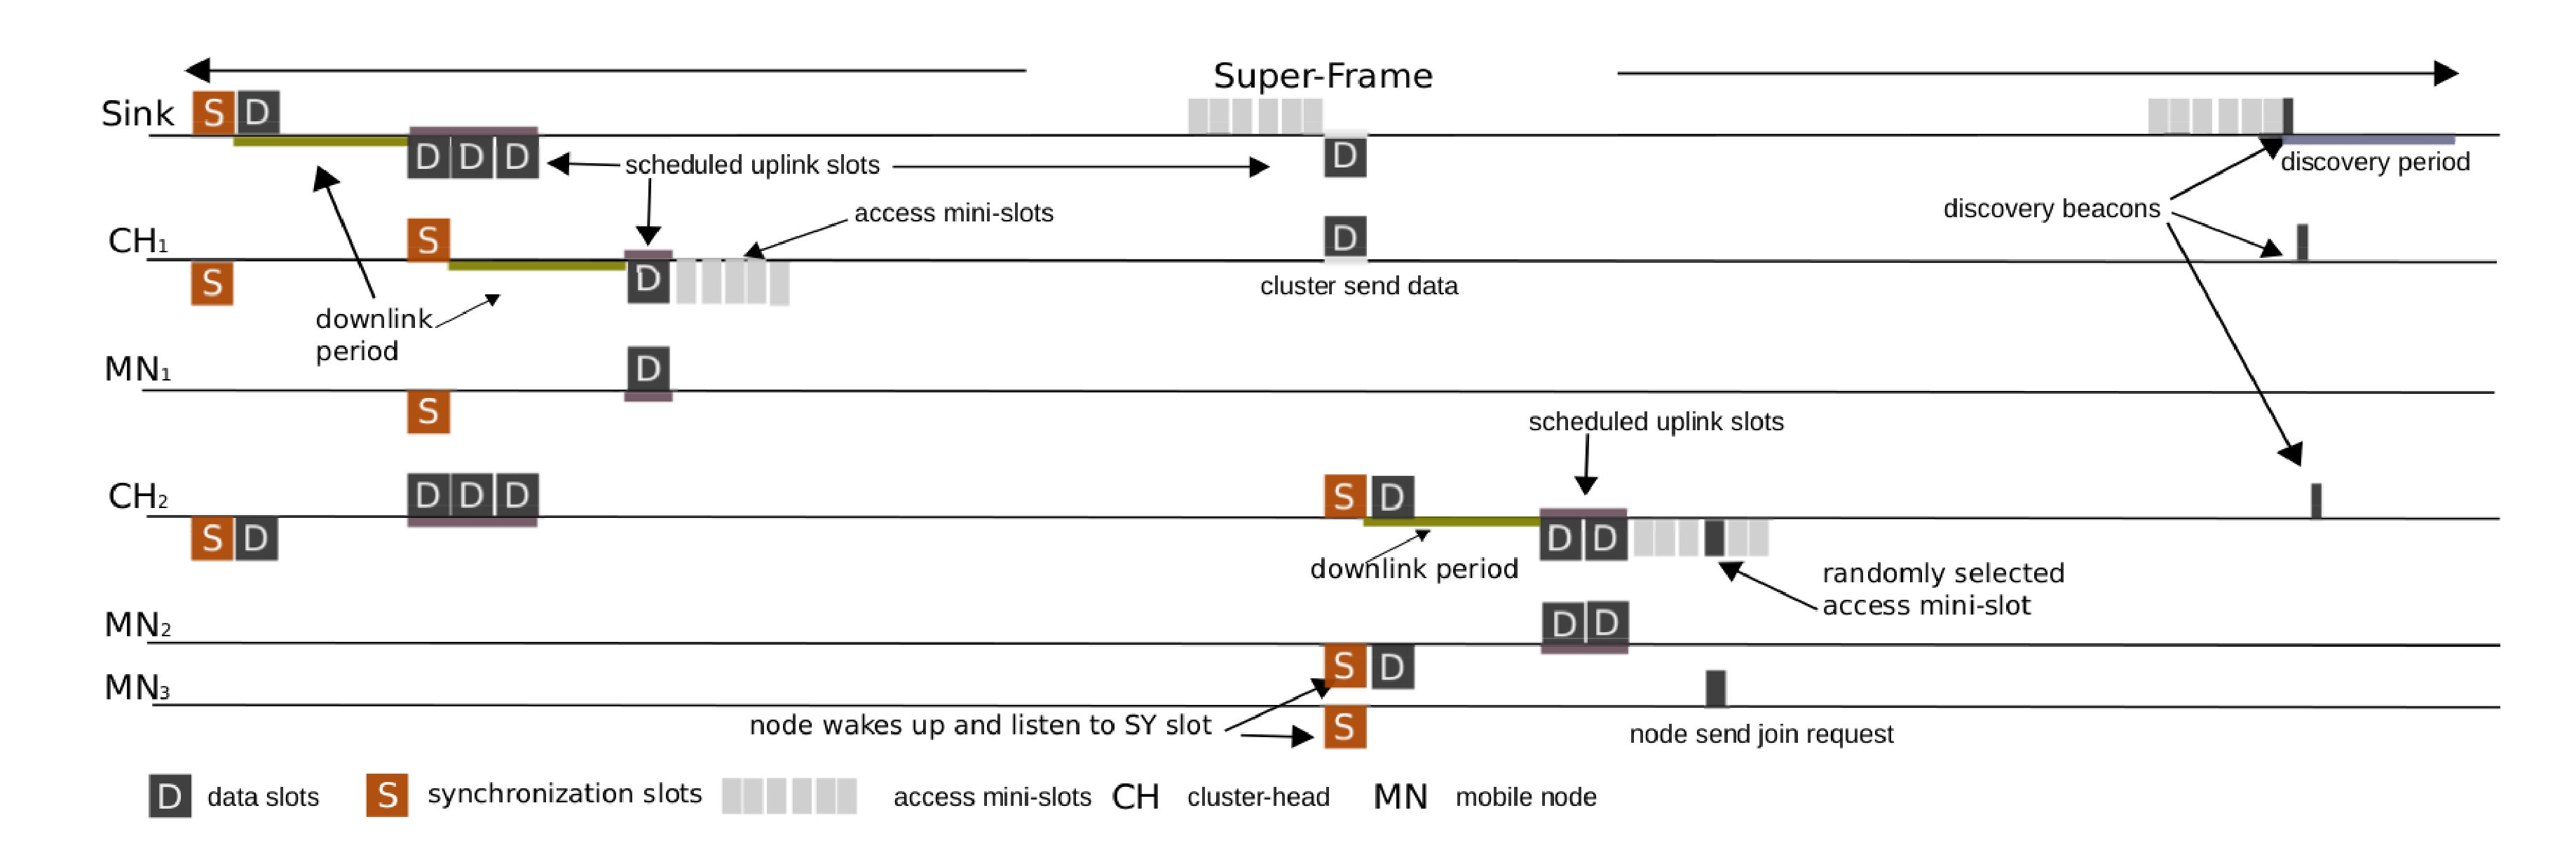
\includegraphics[scale=0.24, natwidth=0.38\textwidth]{mobisense_timing}
		\caption{Mobisense : Timing Diagram}
	\label{fig:mobisense-timing}
  \end{center}
\end{figure}


\subsubsection{Mobisense}
Mobisense \cite{mobisense} is a cross-layer architecture designed for micro-mobility scenarios. It assumes existence of a backbone static network which helps in routing data to the basestation. Each of the static nodes in the network act as a cluster head. Each cluster head operates in a different channel, maintains a cluster of mobile nodes, supports uplink and downlink transmission to and from the basestation. The super-frame is divided into Synchronization, Downlink and Uplink phase, access mini-slots and a discovery slot. During the discovery slot, the cluster head uses a common channel to  advertise information about the cluster. Any mobile node entering the cluster will collect information about the cluster and will send a join request during the access mini-slot. The cluster head adds the new mobile node to the cluster and adapts the schedule for downlink and uplink transmissions and broadcast the schedule information during the synchronization slot.  

\section{Opportunistic Routing}

Conventional routing techniques basically follow best-path routing, which assumes lossless communication links between nodes and a fixed topology. In an ideal wireless network with fixed channel conditions, best-path routing will provide excellant results. But this is not applicable to a Mobile Wireless Sensor network where due to the continuous movement of mobile nodes, the link quality between nodes and the overall topology of the network, continuously kepp changing. Best-path routing provides poor results in those channel conditions. As an alternative, Opportunistic routing gathers information about the current channel conditions and dynamically chooses a next-hop node based on the information. In the following sections we discuss three opportunisitc routing techniques: EXOR\cite{exor}, ROF\cite{rof} and OR-RSSI\cite{or-rssi}.  

\subsection{ROF: Receiver based Opportunistic Forwarding}
ROF is a Receiver-based forwarding technique which allows the receivers of the data packet to contend for forwarding rights before forwarding, instead of calculating and updating a routing path. This approach aims to solve three key problems in opportunistic routing: (i) Collision detection, (ii) Multicast suppression and (iii) Handling Routing voids, which are explained later in this section. The said problems are handled by using an optimized forwarding priority calculation and a dual-channel forwarding contention mechanism. It is assumed that each node in the network is location-aware. 

The first step in ROF is that the sender embeds its location in the data packet and broadcasts it. Each node receiving this packet is a potential forwarder. The receivers calculate a forwarding priority value considering their distance to sender and to that of base station, radio coverage radius and the remaining energy. If the distance between the receiver and the base station is higher than that of the sender and base station, the data packet is ignored. If not, then the receivers contend for forwarding rights in the contention window. The nodes contend by sending an ATF (Application To Forward) packet to the sender, at a particular slot in the contention window. The slot selection is based on the probability of sending ATF at each slot, which is a function of the priority value. 

The forwarding contention mechanism involves use of dual channels i.e. data and control channels. When the sender receives an ATF packet from one of the receiver, it is considered the winner of the forwarding rights and the sender immediately sends a busy tone on the control channel. To complement this process, each receiver after sending an ATF packet, listen to the control channel for a short period of time for a busy tone from the sender. If it hears a busy tone, it becomes aware that it has won the forwarding rights and stops contending immediately, and so does every other node. The use of dual-channel avoid the hidden terminal problem where a receiver node $N_j$, may not hear the ATF packet sent by Node $N_i$ to the sender and hence still contend for rights and sends its own ATF message to sender, causing the multicast problem. 

If collision of ATF packets occurs, the sender will be unable to decode the received message and hence decides that collision has occured. To manage this situation, the sender sends repetitive busy tone on the control channel. On hearing which, the nodes that have sent ATF will send the ATF packets with probability of 1 during the next slot of the contention window. In case the sender has not received any ATF packets for a pre-decided wait time, it assumes a routing void and goes into over-stepping mode. The over-stepping mode follows the same contention process, except that the forwarding priority calculation ignores the distance to base station factor, thus making all nodes receiving the data packet a potential forwarder. 


\subsection{OR-RSSI}
OR-RSSI is an opportunistic routing mechanism for Mobile Wireless Sensor Networks based on RSSI, specifically designed for network with sparse distribution of nodes. This approach calculates an opportunistic probability (OP) based on the RSSI value of beacons periodically sent by base station and the mobility vector(MV). The node with the highest OP wins the forwarding rights. The sink periodically broadcasts beacons with high transmission power. The nodes receiving the beacons, update their OP value based on the RSSI of the beacon. The OP value for node $i$ w.r.t sink $s$, with a mobility vector $\vec{mv_i}$, is calculated based on equation \ref{eqn:orrsi-eqn01}, where $c$ and $\alpha$ are constants. 

\begin{equation}
	OP_{is} \gets OP_{is} + \frac{1}{|RSSI|} \times \alpha + \vec{mv_i} \times c
	\label{eqn:orrsi-eqn01}
\end{equation}

$\alpha$ ia a factor which influences the OP value based on RSSI. Mobility vector is a simple model which represents the movement of the node $i$ w.r.t the sink. $\vec{mv_i} = 1$ if node $i$ is moving towards sink, $\vec{mv_i} = -1$ if it is moving away and $\vec{mv_i} = 0$ otherwise. The 


\begin{figure}[h]{} 
  \begin{center}
		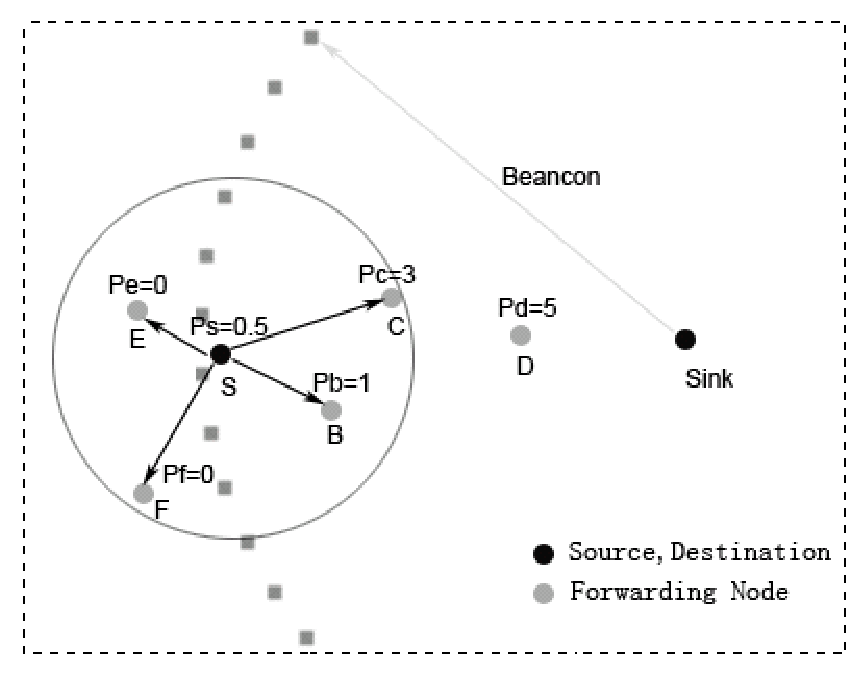
\includegraphics[scale=0.4, natwidth=0.38\textwidth]{orrssi_scenario01}
		\caption{OR-RSSI : Illustration}
	\label{fig:orrsssi-scenario}
  \end{center}
\end{figure}


\section{Time Synchronization}

\subsection{Need for Time Synchronization}
\subsection{Existing Techniques}
\subsubsection{RBS: Reference Broadcast Synchronization}
\subsubsection{TSPN: Timing-sync for sensor networks}
\subsubsection{FTSP: Flooding Time Synchronization Protocol}

\section{Mobility Estimation}
\subsection{Challenges}
\subsection{Techniques}





 
% Chapter 1

\chapter{Proposal} % Main chapter title

\label{prop} % For referencing the chapter elsewhere, use \ref{Chapter1} 

\lhead{Proposed Approach} % This is for the header on each page - perhaps a shortened title
Considering the fact that energy efficiency is the primary goal of any wireless sensor network application, we have designed DS-MMAC, Dynamic Schedule based MAC protocol for Mobile Wireless sensor network. It should be noted that DS-MMAC is specifically designed for mixed deployment of sensor nodes (mobile and static). It is assumed that a dense random deployment of static nodes is available. This approach is a pure MAC protocol i.e. routing is handled separately. Routing is handled separately using a modified version of AODV \cite{aodv}. Based on our performance evaluation of DS-MMAC, we observe that it performs very under in a mixed deployment scenario with mobile nodes moving at low velocities. The algorithm is explained in detail in the following sections. We have simulated DS-MAC and compared the results against Hybrid MAC \cite{hmac} in Chapter \ref{simulacra}. 

As a continuation of DS-MMAC, we have also designed a Cross Layer Architecture for a strictly mobile sensor network, CA-MOBILE. Unlike DS-MMAC, CA-MOBILE inherently handles routing by forwarding data packets to a node which is closest or potentially close to the base station. The key aspects of this approach are Dynamic Cluster Head Election, Multi-channel Data Transfer and Mutually Beneficial Forwarder Assignment. Inspired by opportunistic routing techniques \cite{exor}\cite{rof}, we have designed CA-MOBILE to forward packets by dynamically choosing a forwarder for each source node, using updated mobility information of the cluster. It should be noted that even though the initial simulation results of CA-MOBILE are promising, It is not yet analyzed w.r.t to all the network parameters (scalability, reliability, packet delivery ratio, energy efficiency). 

\section{DS-MMAC}

We propose a MAC protocol that uses dynamic scheduling to handle the mobile nodes in the network. Each frame is divided into control phase, for managing the mobile nodes, data transfer phase for collecting data from the mobile nodes and routing phase during which the static node forwards the aggregated data to the next node based on an established routing path \cite{aodv}. We employ request-reply mechanism for data transfer, which not only improves the reliability of the data transfer but also serves as a means to inform the mobile nodes about their wake up time during the next frame. The primary goal of our protocol design is to improve energy efficiency by increasing the sleep time of the mobile nodes. The request-reply mechanism also ensures that collision does not happen when a mobile node moves from one virtual cluster \cite{smac} to another. The local schedule maintained by each static node in the network, is designed to be flexible that it keeps on changing based on network traffic and the mobility of the neighbors.

\subsection{Problem Statement and Assumptions}
Accommodating mobile sensor nodes in the sensor network introduces a few challenges for the network protocol designers. Due to the rapid movement of mobile nodes, the topology of the entire network changes every instant. Designing a MAC and/or routing protocol for a network with dynamic topology is a challenging task. An efficient routing algorithm in this case, essentially requires efficient medium access, with minimum packet loss. Contention based algorithms increase the network overhead and also the probability of collision is high. Hence, this scenario requires a TDMA based MAC protocol which dynamically adapts to the changes in the mobile node traffic in the neighborhood.  

We assume that a dense unstructured deployment of static nodes is available in the network for routing data to the base station. It is also assumed that the cluster head possesses the ability to aggregate data before forwarding to the base station.

\subsection{Algorithm}

\subsubsection{Network Initialization}
The first phase of our approach is Network initialization, during which the static nodes in the network exchange timing slots to communicate with each other. This process of offering a TDMA slot to a static node starts from the base station. It should be noted that none of the static nodes start communication with their mobile neighbors before acquiring a routing slot from their parent. The base station starts off the process by sending different timing slots to all its \emph{children} i.e., one hop static neighbors. The children randomly choose a time slot, different from the one offered to them by the base station and enable their one hop static neighbors(grand children). This process continues until all the nodes acquire a routing slot from their parents. Meanwhile, the nodes which are enabled by their parents, start communicating with their mobile neighbors. Once a mobile node starts receiving data from its neighbors, it starts aggregating the data. This aggregated data is forwarded to its parent during the routing slot offered by its parent, which eventually reaches the base station.


The communication with mobile nodes involves two stages : Control Phase and Data phase. Control phase is organized into (i) Discovery Request Phase (ii) Discovery Reply Phase and (iii) Schedule phase, which are explained clearly in the following sections:

%\subsubsection{Control Phase}
Control Phase is organized into (i) Discovery Request Phase, (ii) Discovery Reply Phase and (iii) Schedule phase.

\subsubsection{Discovery Request Phase}
\label{disc_req_phase}
During the start of the frame, the cluster head broadcasts a discovery request packet \emph{disc\_req}. The discovery request packet is an advertisement message broadcasted by the cluster head to inform the mobile nodes in the neighborhood about the cluster. This message contains valuable information regarding the cluster including cluster size and remaining energy. Also, a mobile node receiving this message can estimate the approximate distance between the cluster head and itself, based on the RSSI value acquired from the radio message. It is possible that a mobile node may receive more than one disc\_req message from more than one cluster head. In that case, the mobile node chooses a cluster based on the current cluster size, remaining energy of the cluster head and the distance between the cluster head and itself.

\begin{figure}[h]{} % Inline image example
  \begin{center}
   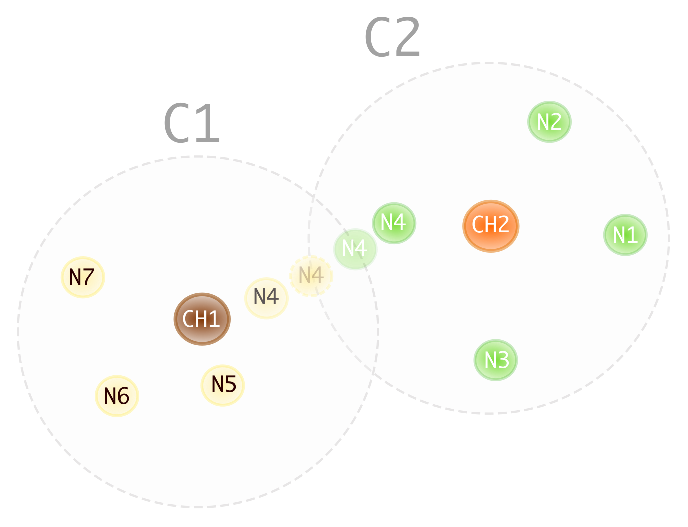
\includegraphics[scale=0.7, natwidth=0.38\textwidth]{scenario01}
	 \caption{A sample scenario}
	 \label{fig:scenario01}
  \end{center}
\end{figure}


\subsubsection{Discovery Reply Phase}
\label{disc_rep_phase}
The Discovery Reply Phase consists of a finite number of slots during which the cluster head listens for Discovery Reply packets \emph{disc\_rep} from the mobile nodes. The mobile node, after choosing a cluster to join, wakes up during a random slot in the Discovery Reply slots and sends a \emph{disc\_rep} packet to the cluster head. The slot selection as mentioned above, is randomly done by the mobile node. The maximum number of these slots is \emph{x} which depends on the node density in the network.

\begin{equation}
	x = m\pi r^2 
	\label{eqn:x}
\end{equation}

$m$: Density of mobile nodes, $r$: Radio coverage radius of static nodes\\

\subsubsection{Schedule Phase}
\label{sched_phase}
Based on the \emph{disc\_req} packets received in the previous section, the cluster head builds a schedule for the mobile nodes to communicate with it. The order of frame access to nodes in this schedule is based on the order of reception of \emph{disc\_rep} packets. The schedule is broadcasted by the cluster head during this phase. It should be noted that any node which issued a join request in this round should be in listen mode during this phase, to receive the schedule packet. 

\begin{figure}[h]{} 
  \begin{center}
    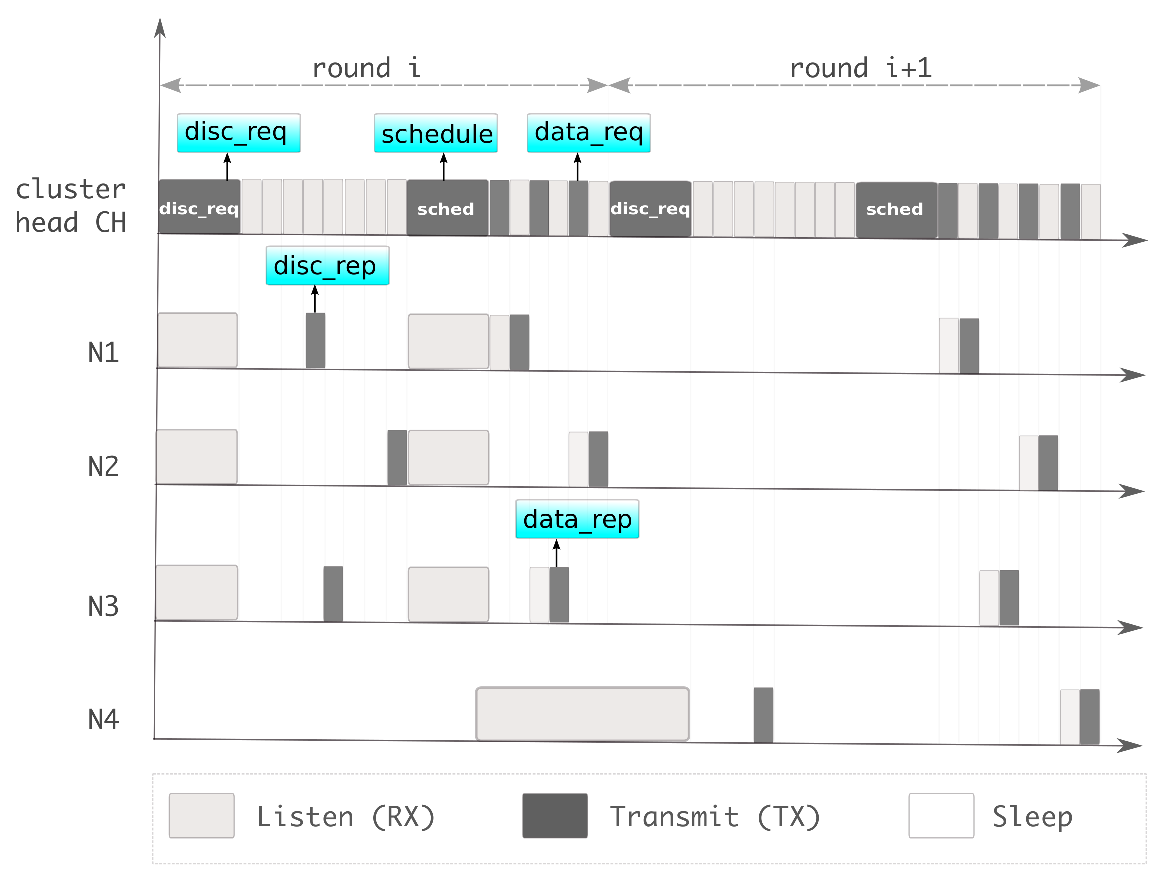
\includegraphics[scale=0.6, natwidth=0.38\textwidth]{timing-dia}
  \end{center}
  \caption{Time line Showing the Cluster head communication}
	\label{fig:timing}
\end{figure}


\subsubsection{Data Phase}
\label{data_phase}

From the schedule message, each mobile node acquires its data slot for communication with the cluster head. The data phase is divided into pairs of \emph{data\_req} and \emph{data\_rep} slots. Each pair serves one mobile node. When a mobile node wakes up during its data slot, it receives a \emph{data\_req} message from the cluster head. The cluster head embeds a time value \emph{$t_1$} in this message, which represents a time in the future (next frame) when the corresponding mobile node should wake up for the next data transfer session. The mobile node after receiving this message sends a \emph{data\_rep} message to the cluster head, set a timer to wake up after \emph{$t_1$} seconds and puts the radio in sleep mode. 

%To understand our approach, let's consider the scenario depicted in figure \ref{fig:scenario}. There are two clusters $C_1$ and $C_2$. Each cluster consists of a few mobile nodes and a cluster head (CH$_1$,CH$_2$). 

Consider the scenario given in figure \ref{fig:scenario01}, where CH$_1$ and CH$_2$ are cluster head of clusters $C1$, $C2$ respectively. Node \emph{$N_4$} moves from $C_1$ to $C_2$. When N4 moves out of the range of CH$_1$, it stops receiving the periodic data request message from CH$_1$. Realizing that it has moved out of cluster $C_1$, N4 switches its radio to listen mode, listening for \emph{disc\_req} packet from other cluster heads.
After waiting a while, it receives a \emph{disc\_req} message from CH$_2$ as shown in figure \ref{fig:timing}. N4 chooses one of the slots in the discovery reply phase to send a \emph{disc\_rep} packet. CH$_2$ adds N4 to the schedule and broadcast the schedule. N4 acquires its data transfer slot timing from the schedule. During its slot, N4 wakes up to receive \emph{data\_req} packet from CH$_2$ and replies to it with a \emph{data\_rep} packet. Using the next data transfer session schedule acquired from the \emph{data\_req} packet, N4 sets a timer and puts its radio in sleep mode.

The algorithm followed by the mobile nodes in our approach is mentioned in Algorithm \ref{algo:mob}. Initially mobile node will switch on its radio to RX state and listens for $disc\_req$ packets from cluster heads. When it receives a $disc\_req$ it binds itself to the cluster head and sends a $disc\_rep$ packet to the cluster head, depicted in lines 2 to 7 in Algorithm \ref{algo:mob}. After which it waits for a $sched$ packet from the cluster head. The mobile node extracts its scheduled slot from $sched$. Based on which, it wakes up and listens for a $data\_req$ packet from the cluster head as given in lines 15,16. Line 17 to 19 describes the data request and response mechanism. The $data\_req$ message also contains the slot during which the mobile node should wake up during the next frame. 


%%%%%%%%%%%%%%%%%%%%%%%%%%%%%%%%%%%%%%%%%%%%%%%%%%%%%%%%%%%%%%%%%%
%\iffalse 
%In this section we will discuss the working of our protocol from a mobile node and from a static node's perspective. 
%
%--- Try framing an algorithm w.r.t the static node. \\
%
%Try framing an algorithm w.r.t the mobile node. \\
%
%Try framing an algorithm w.r.t the timeslot allocation b/w the static node during the network initialization. \\ \\

% ------------------------------------------------------- %
\alglanguage{pseudocode}
\begin{algorithm}[H]
	\caption{From Mobile Node's Perspective}
	\label{algo:mob}
\begin{algorithmic}[1]
	\Procedure {DS-MMAC\_MOBILE}{}%{$P_c$, $N$, $R$, $a$, $\Re$}
	\While{\emph{true}}
%\State toRadioLayer(RX\_STATE)
\If {\emph{receive($disc\_rep$)}}
	\State $CH\gets disc\_rep.source$
	\State $disc\_slot\gets rand()$
	\State \emph{Wake up at $disc\_slot$}
	\State $send(disc\_rep)$
%	\State toRadioLayer(RX\_STATE)
	\If {\emph{receive(Sched)}}
	\For{$i = 0 \rightarrow Sched.node\_count$}
	\If { Sched.node\_id = ADDR }
	\State $data\_slot \gets Schedule[i].slot$
%	\State toRadioLayer(SLEEP\_STATE)
	\State break
	\EndIf
	\EndFor
	\State \emph{Wake up at $data\_slot$}
%	\State toRadioLayer(RX\_STATE)
	\While{\emph{receive(DataReq)}}
	\State $data\_slot \gets DataReq.slot$
	\State $send(DataRep,CH)$
	\State \emph{Wake up at $data\_slot$}
%	\State toRadioLayer(RX\_STATE)
	\EndWhile
	\EndIf
\EndIf
\EndWhile
\EndProcedure
\end{algorithmic}
\end{algorithm}
%\fi

Algorithm \ref{algo:ch} describes our approach from a cluster head's perspective. The cluster head initiates the communication by broadcasting a $disc\_req$ message and then waits for the nodes in its vicinity to respond with a $disc\_rep$ message. The cluster head stores the addresses of the nodes sending the $disc\_rep$ message in a local buffer \emph{boundNodes}. This process is described in lines 3 to 7. Based on the contents of the buffer, the cluster head builds and broadcasts the schedule for this frame. Lines 13 to 20 depicts how the cluster head services the mobile nodes. It should be noted that in each $data\_req$ message, the cluster head embeds the slot information on when the mobile node should wake up during the next frame.





%%%%%%%%%%%%%%%%%%%%%%%%%%%%%%%%%%%%%%%%%%%%%%%%%%%%%%%%%%%%%%%%%%
\alglanguage{pseudocode}
\begin{algorithm}[H]
	\caption{From Cluster Head's Perspective}
	\label{algo:ch}
\begin{algorithmic}[1]
	\Procedure {DS\_MMAC\_MOBILE}{}%{$P_c$, $N$, $R$, $a$, $\Re$}
	\While{\emph{true}}
%\State toRadioLayer(RX\_STATE)
\If {\emph{receive($disc\_req$)}}
	\State $broadcast(disc\_req)$
	\While{receive(disc\_rep)}
		\State \emph{bound\_nodes.add(disc\_rep.source)}
	\EndWhile
	\For{$i = 0 \rightarrow bound\_nodes.size$}
		%\State $sched.node\_id[i] = boundNodes[i]$
		%\State $sched.slot[i] = 2 \into i + FRAME\_SIZE$
		\State \emph{/* add to schedule */}
	\EndFor
	\State \emph{broadcast(sched)}
	\For{$j = 0 \rightarrow bound\_nodes.size$}
		\State $DataReq.slot \gets next\_slot()$
		\State \emph{send(data\_req,bound\_nodes[j]}
		\If {\emph{receive(data\_rep)}}
			\State \emph{store data\_rep}
		\Else\ \emph{boundNodes.remove(j)}
		\EndIf
	\EndFor
\EndIf
\EndWhile
\EndProcedure
\end{algorithmic}
\end{algorithm}
%

The simulation of DS-MMAC s done and the results are compared with Hybrid MAC proposed in \cite{hmac}. A thorough performance evaluation of DS-MMAC is done and it is described in Chapter \ref{simulacra}.


\section{CA-MMAC}
We propose a Cross Layer Architecture for strictly Mobile WSN that uses mobility parameters of nodes to manage data forwarding in the network. Our algorithm organizes the network into clusters based on geographical location of nodes. Cluster information is updated every round. Each cluster consists of a cluster head which is elected using the standard cluster head election mechanism proposed in \cite{leach}. Cluster head re-election is done when the current cluster head finds a more suitable candidate for the task. During each round the cluster head acquires the mobility information(location,velocity) of the cluster members. Based on the collected information, it assigns a forwarder node for each node with data packets to forward. The assignment is designed in such a way that each node is able to complete the data transfer based on the size of data it contains and also considering the location and velocity of the forwarders chosen. We have discussed the assignment problem in depth in Section \ref{assgn_prob}.


\subsection{Problem Statement}

In a fully mobile Wireless Sensor Network, data forwarding from a sensor node to the base station involves a number of challenges. Mobility of nodes leads to a condition where the links established between nodes changes dynamically. Due to the constant change in link quality, the choice the best node to forward data should consider the mobility parameters of the node. The parameters to be considered are the location of the mobile node w.r.t. to the base station and the source(or the current forwarder). This scenario requires an opportunistic routing protocol which assigns forworders to source nodes based on their mobility parameters.

\subsection{Assumptions}
\begin{itemize}
	\item The network consists of a dense random deployment of mobile nodes 
	\item All nodes are aware of their location and their current velocity
	\item Nodes have the ability to aggregate data before forwarding
	\item Location of basestation is fixed and is known to all the nodes
\end{itemize}


\subsection{Assignment Problem}
\label{assgn_prob}
In the figure, all the nodes inside the gray circle belong to a cluster, $C_1$. CH is their cluster head. The cluster head is responsible for managing the data transfer within the cluster. When a node \emph{N1} has data to send to basestation, it sends a \emph{RTS} (Ready To Send) message CH and now, its CH's responsibility to find a suitable node, \emph{$N_i$} for \emph{N1} to forward its data. We need to consider parameters such as the velocity (direction and speed), distance from the base station, distance from the source/sender node and the contact time between N1 and the $N_i$. Contact time is basically the period during which N1 and $N_i$ are within the range of each other. The first part of the problem is to build a model using the given parameters, using which a node's suitability for forwarding data will be quantified. \\

\begin{figure}[h]{} 
  \begin{center}
		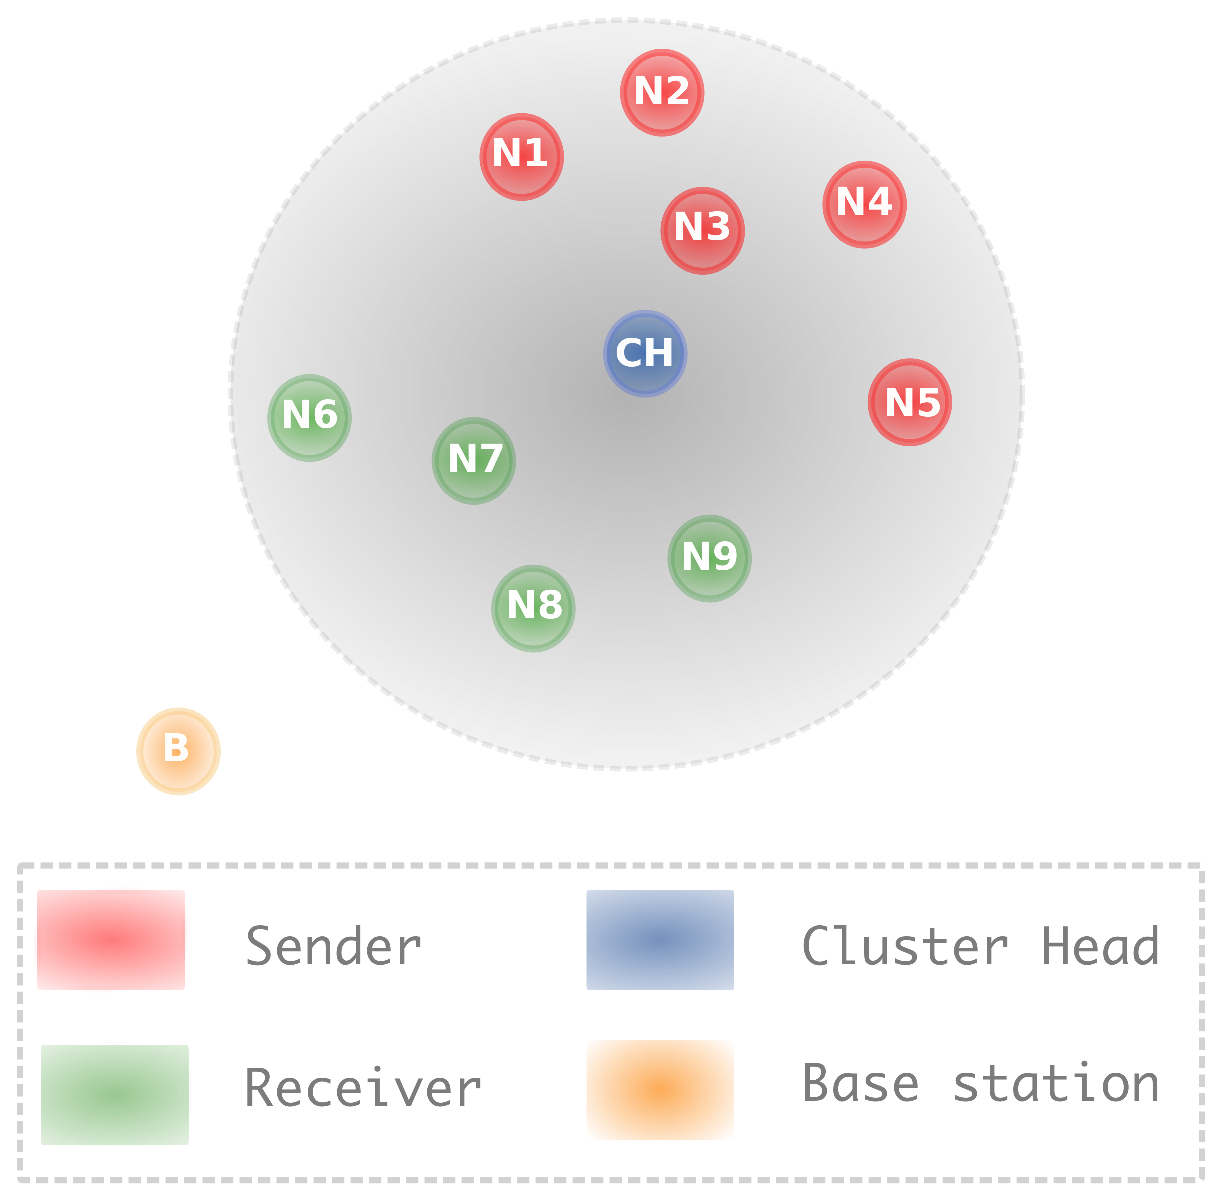
\includegraphics[scale=0.4, natwidth=0.38\textwidth]{ca_mmac_scenario01}
		\caption{Assignment Problem}
	\label{fig:scenario02}
  \end{center}
\end{figure}


The second part of the problem is to decide which destination nodes to assign to which source nodes, based on the model. Assume that the nodes $N_1, N_2, N_3$ and $N_5$ have data to forward to base station and the nodes N6, N7, N8 and N9 are the candidates for destination node. This becomes an assignment problem; which nodes to assign to which nodes?

\subsection{Algorithm}

The first step in our algorithm is Cluster head election. Every node randomly backs off and then broadcasts a $sync$ message. The nodes receiving the $sync$ message, become the cluster members, while the node broadcasting becomes the cluster head. In case of collision of $sync$ message, the process of random back-off and broadcast is repeated. This constitutes the network setup phase. Data gathering and opportunistic forwarding take place in the subsequent phases. Each round in CA-MMAC consists of the following phases: (i) Synchronization (ii) Meta phase (iii) Schedule (iv) Data Phase, which are explained in detail in the following sections. It should be noted that except the data phase, in all the other phases, a common channel is used for communication. 

\subsubsection{Synchronization}
During the synchronization phase, the cluster head broadcasts the $sync$ message, which consists of the cluster information including the cluster size and the centroid of the cluster.  The $sync$ message acts as an advertisement for the new nodes joining the cluster. 

\subsubsection{Meta Phase}
After synchonization, we have meta phase which is split into small slots named meta slots, illustrated in \ref{fig:ca-timing}. The cluster members choose a random meta slot for sending $meta$ packets to the cluster head. The $meta$ packet consists of mobility information of the node incluing current location and velocity. Optionally the cluster members which have data to forward, can embed a Request To Send, $rts$ message along with the $meta$ packet. The cluster head updates the mobility information of the cluster during the meta phase. It then uses this information to decide which node forwards data to which node.

\begin{figure}[h]{} 
  \begin{center}
		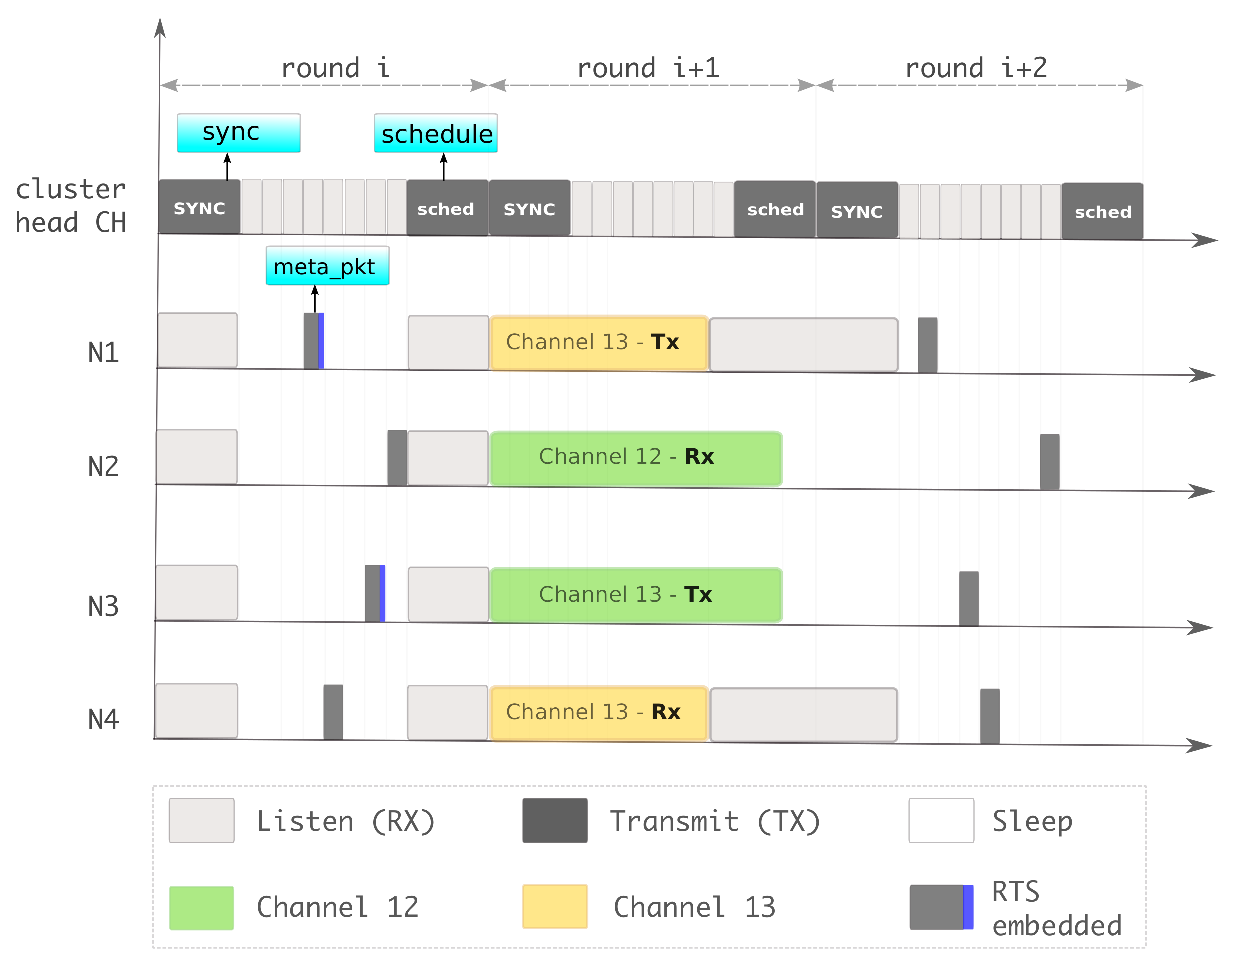
\includegraphics[scale=0.6, natwidth=0.38\textwidth]{ca-timing}
		\caption{Timing Diagram}
	\label{fig:ca-timing}
  \end{center}
\end{figure}


\subsubsection{Schedule}
Baed on the mobility information of the cluster, the cluster head first calculates the distance between each node and the centeroid and the velocity of nodes and decides if the cluster needs a new cluster head. If it chooses a new cluster head, it embeds this message along with the $sched$ packet.  The nodes receiving this message will become aware of the new cluster head, and wait for the next $sync$ message from the newly chosen cluster head, after the end of this frame. The schedule basically consists of data pairs and data channels. The cluster head dynamically chooses a forwarding node for each source node based on the assignment algorithm explained in \ref{assgn_prob}. It also assigns an unique channel over which the data transfer between the corresponding data pair is intended to occur. The nodes receiving the $sched$ message, change their local cluster head variable to the new cluster head's id, in case the cluster head has also sent a new cluster head along with the schedule. By iterating through the schedule, the cluster member comes to know about its data pair and starts data transfer on the assigned channel.

\subsubsection{Data Phase}
The data transfer is designed to include acknowledgement, \emph{ACK} for higher reliability. The receiver keeps track of the RSSI (Receiver Signal Strength) of the data packets sent by the sender, based on which an approximate distance between them is calculated. If this distance crosses a threshold, the receiver sends a \emph{NACK} message to the sender in place of \emph{ACK} Upon receiving the \emph{NACK} message, the sender stops the data transfer and goes to sleep. It continues the data forwarding during the next round, when the cluster head assigns a new forwarding node to it.\\

\alglanguage{pseudocode}
\begin{algorithm}[H]
	\caption{CA-MOBILE : Algorithm}
	\label{algo:ca-mobile}
\begin{algorithmic}[1]
	\Procedure {CA\_MOBILE}{}%{$P_c$, $N$, $R$, $a$, $\Re$}
	\State \emph{/* Random Back-Off */}
	\If {\emph{receive(sync)}}
	% cluster member
	\State $cluster\_head \gets sync.source$
	\While{\emph{true}}
		\State $meta\_slot \gets rand()$
		\State \emph{Wake up at $meta\_slot$}
		\State $meta.mob\_vector \gets self\_mob\_vector()$
		\If {\emph{hasData()}}
			\State $meta.rts \gets true$
		\EndIf
		\State $send(meta)$
		\If {\emph{receive(sched)}}
		\For{$j = 0 \rightarrow sched.node\_count$}
			\If { sched.node\_id = SELF }
				\State $data\_pair \gets sched[i].data\_pair$
				\State $data\_channel \gets sched[i].data\_channel$
			\EndIf
		\EndFor
		\State \emph{/* Switch to data\_channel */}
		\State \emph{/* Initiate data transfer */}
		\EndIf
		\State {\emph{receive(sync)}}
	\EndWhile
	\Else
	\While{\emph{true}}
		\State $broadcast(sync)$
		\While{receive($meta$)}
			\State \emph{bound\_nodes.add(meta.source)}
			\State \emph{mobility\_vector.add(meta.mob\_vector)}
		\EndWhile
		\State $new\_cluster\_head \leftarrow min(boundNodes,centroid)$
		\State $sched.embed(new\_cluster\_head)$
		\For{$i = 0 \rightarrow bound\_nodes.size$}
			\State \emph{/* Assign data pair, data channel, add to schedule */}
		\EndFor
		\State \emph{broadcast(sched)}
			\Else\ \emph{boundNodes.remove(j)}
	\EndWhile
	\EndIf
\EndProcedure
\end{algorithmic}
\end{algorithm}
 
% Chapter 1

\chapter{Simulation and Results} % Main chapter title

\label{simulacra} % For referencing the chapter elsewhere, use \ref{Chapter1} 

\lhead{Simulation and Results} % This is for the header on each page - perhaps a shortened title

%----------------------------------------------------------------------------------------

\section{Simulator used}
Write in detail about Castalia - justify use of Castalia

% Add Param table

\section{Performance Evaluation}

%Write about Simulation scenario

For evaluating the performance of DS-MMAC, we have compared the results of the proposed approach with Hybrid MAC\cite{hmac}. Simulation is done in Castalia, an omnetpp based framework for low power networks with realistic radio propagation models and analysis tools \cite{castalia}. The parameters chosen for comparison are listed in Table \ref{sim_para}.

We have considered a simulation area of $100 \times 100m$ where an unstructured deployment of sensor node is done. The mobile nodes are initially distributed evenly across the simulation area. The mobile nodes follow the Random Waypoint mobility model and move at a constant velocity. The simulation was run for 1000 seconds. Simulation was done by varying the number of mobile nodes and by varying the velocity of the node.


\begin{table}[h]\scriptsize
\begin{center}
\caption{Simulation Parameters}
\label{sim_para}
    \begin{tabular}{ | l |p{3cm} |}
    \hline
Parameters & Values \\  \hline
Network Size & $100 \times 100 $ $m^2$ \\ \hline
Number of Static Nodes & $25$ \\ \hline
Communication radius & $30m$ \\ \hline
Velocity & 2m/s \\ \hline
Number of Mobile Nodes & 1 to 70 \\ \hline
Packet size & 128byte \\ \hline
Simulation Time & 1000Sec \\ \hline
    \end{tabular}
\end{center}
\end{table}


Network lifetime is the deciding factor in any network protocol design in Wireless Sensor Networks. Energy consumption of the proposed protocol was compared against the Hybrid MAC protocol. The results plotted in Figure \ref{fig:em} was done by changing the number of mobile nodes from one to fifteen with a velocity value 2m/s. From the results, it is observed that the power consumption of mobile nodes in our approach is substantially lower than that of Hybrid MAC. This is because of the increase sleep time of mobile nodes in the DS-MMAC approach.\\
\begin{figure}[h]{} 
  \begin{center}
		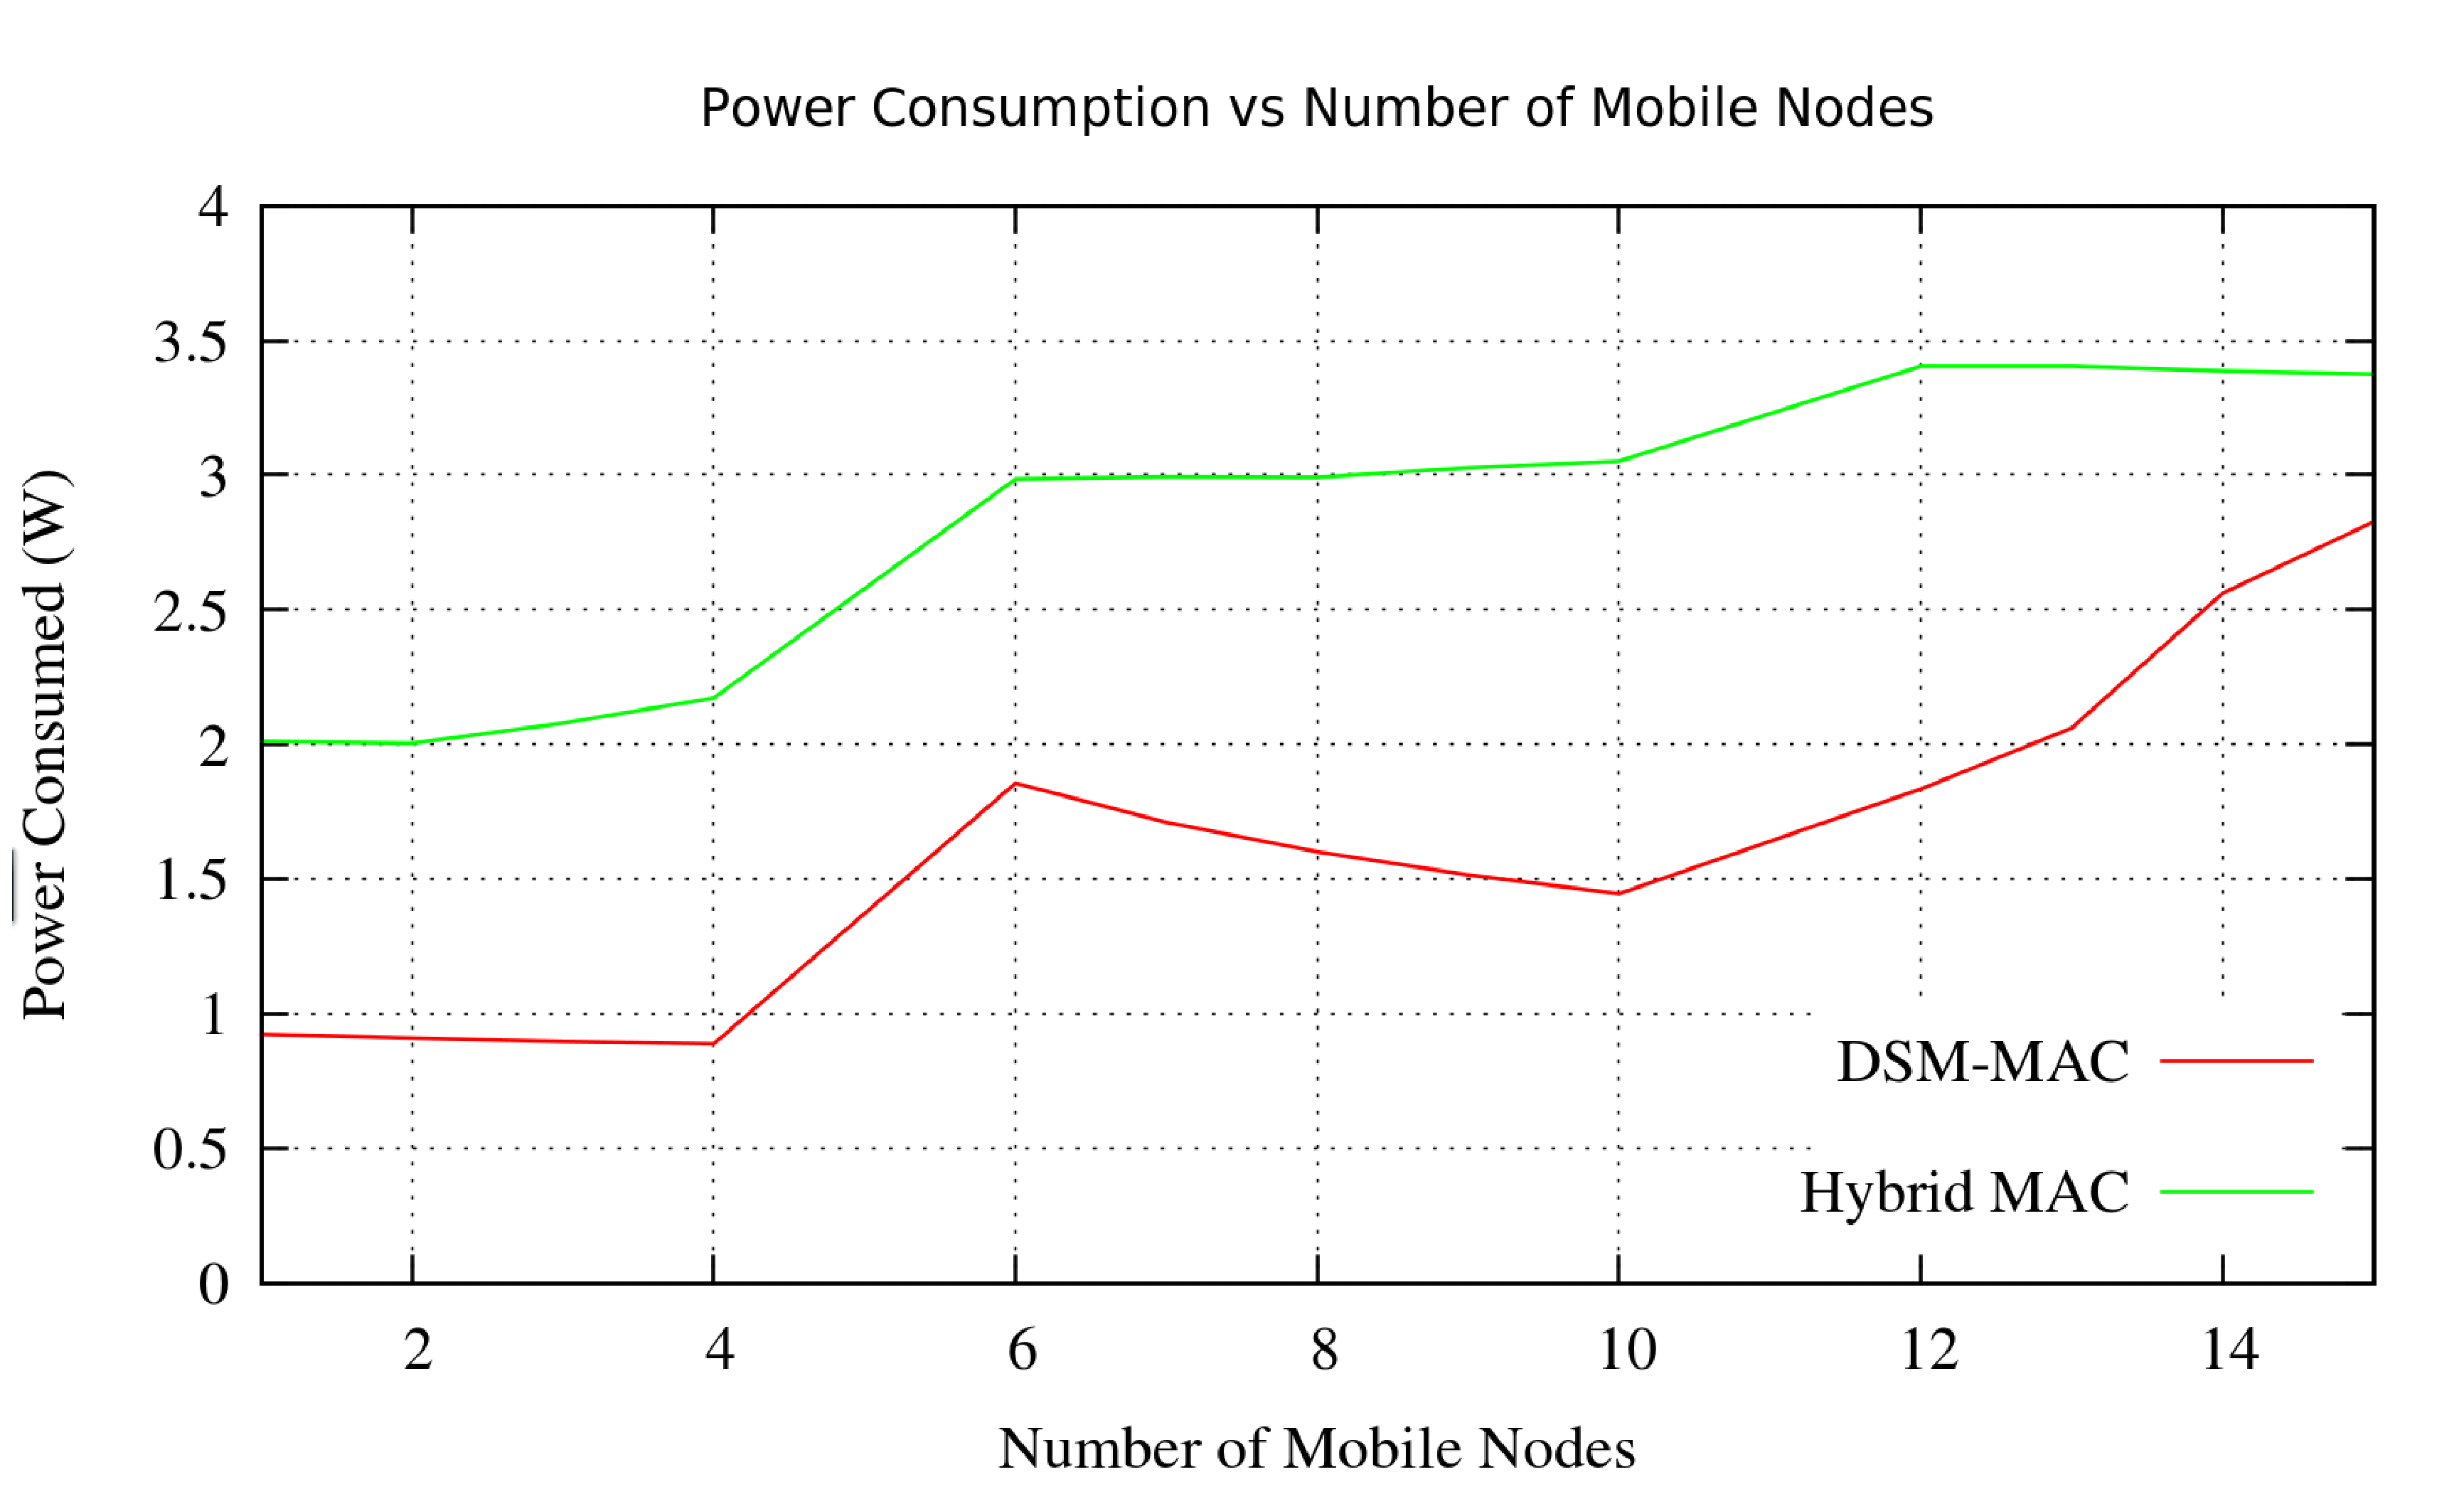
\includegraphics[ width=8.5cm,height=6cm]{em}
  \end{center}
	\caption{Power Consumption vs Number of Mobile Nodes}
		\label{fig:em}
\end{figure}

The Packet delivery ratio is basically the ratio of the number of packets sent to the number of packets received. Figure \ref{fig:PDR} shows the difference in delivery ratio w.r.t to the number of mobile nodes.  Simulation is done for a maximum of 70 mobile nodes.  Hybrid MAC protocol performs slightly better when compared to the proposed approach. Since the neighboring clusters operate on the same channel, the channel interference is high and hence the delivery ratio decreases.
\begin{figure}[h]{} 
  \begin{center}
    		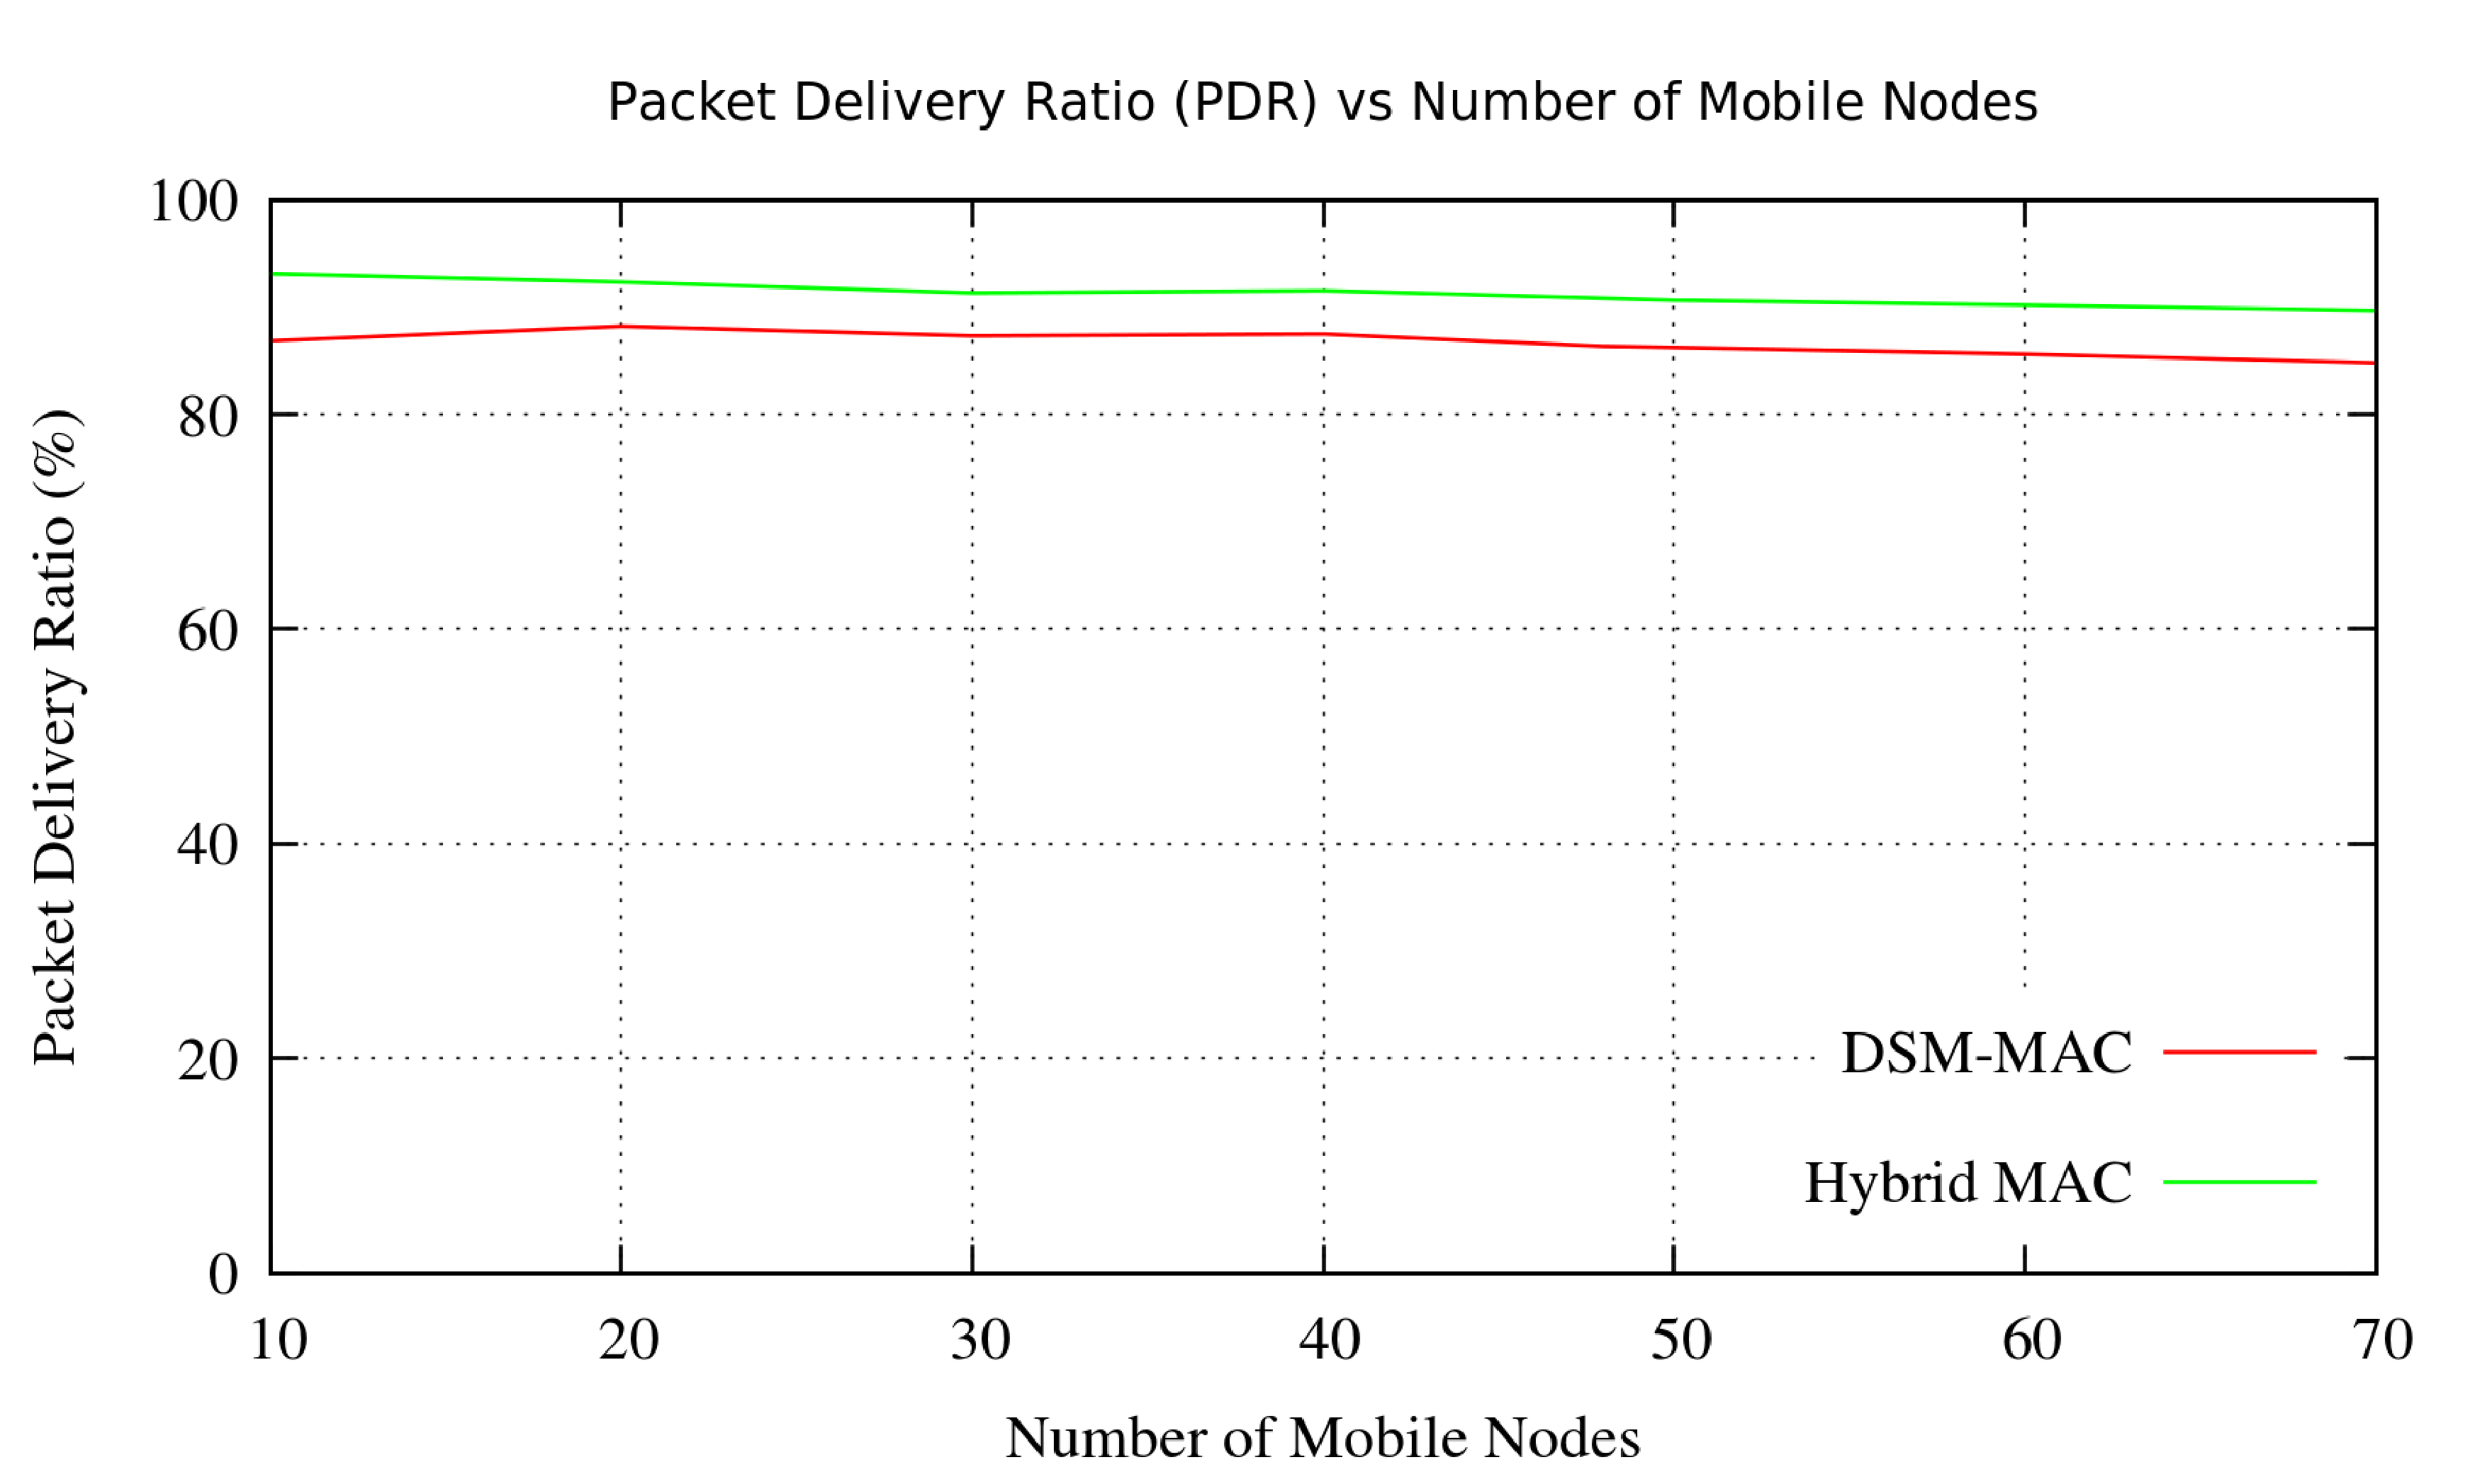
\includegraphics[ width=8.5cm,height=6cm]{prm}
  \end{center}
	\caption{PDR vs Number of Mobile Nodes}
	\label{fig:PDR}
\end{figure}

 Even though the packet delivery ratio is less, the number of packets transmitted and received per second is higher in DS-MMAC approach. This is because of the number of rounds (iteration) per unit time is higher for the same number of mobile nodes. Hence the number of packets send and received per unit time is also higher. This is clear in the Figure \ref{fig:pm}. Figure \ref{fig:pm} shows the relation between the number of packets received per unit time at MAC layer w.r.t the number of mobile nodes. It is clear that the number of packets received is higher in DS-MMAC approach.  But it is a reasonable tradeoff for reduced power consumption and increased throughput. It is a reasonable tradeoff for reduced power consumption and increased throughput. Multichannel based MAC layer implementation for data communication can help in improving the packet delivery ratio.  
 Simulations were done to compare the number of packets delivered w.r.t the velocity of the mobile node. This is done by varying the velocity from $1$ to $10$ m/s. As shown in the Figure \ref{fig:pv}, our approach gives a considerable increase in the number of packets delivered when compared to Hybrid MAC approach. \\

\begin{figure}[h]{} 
  \begin{center}
		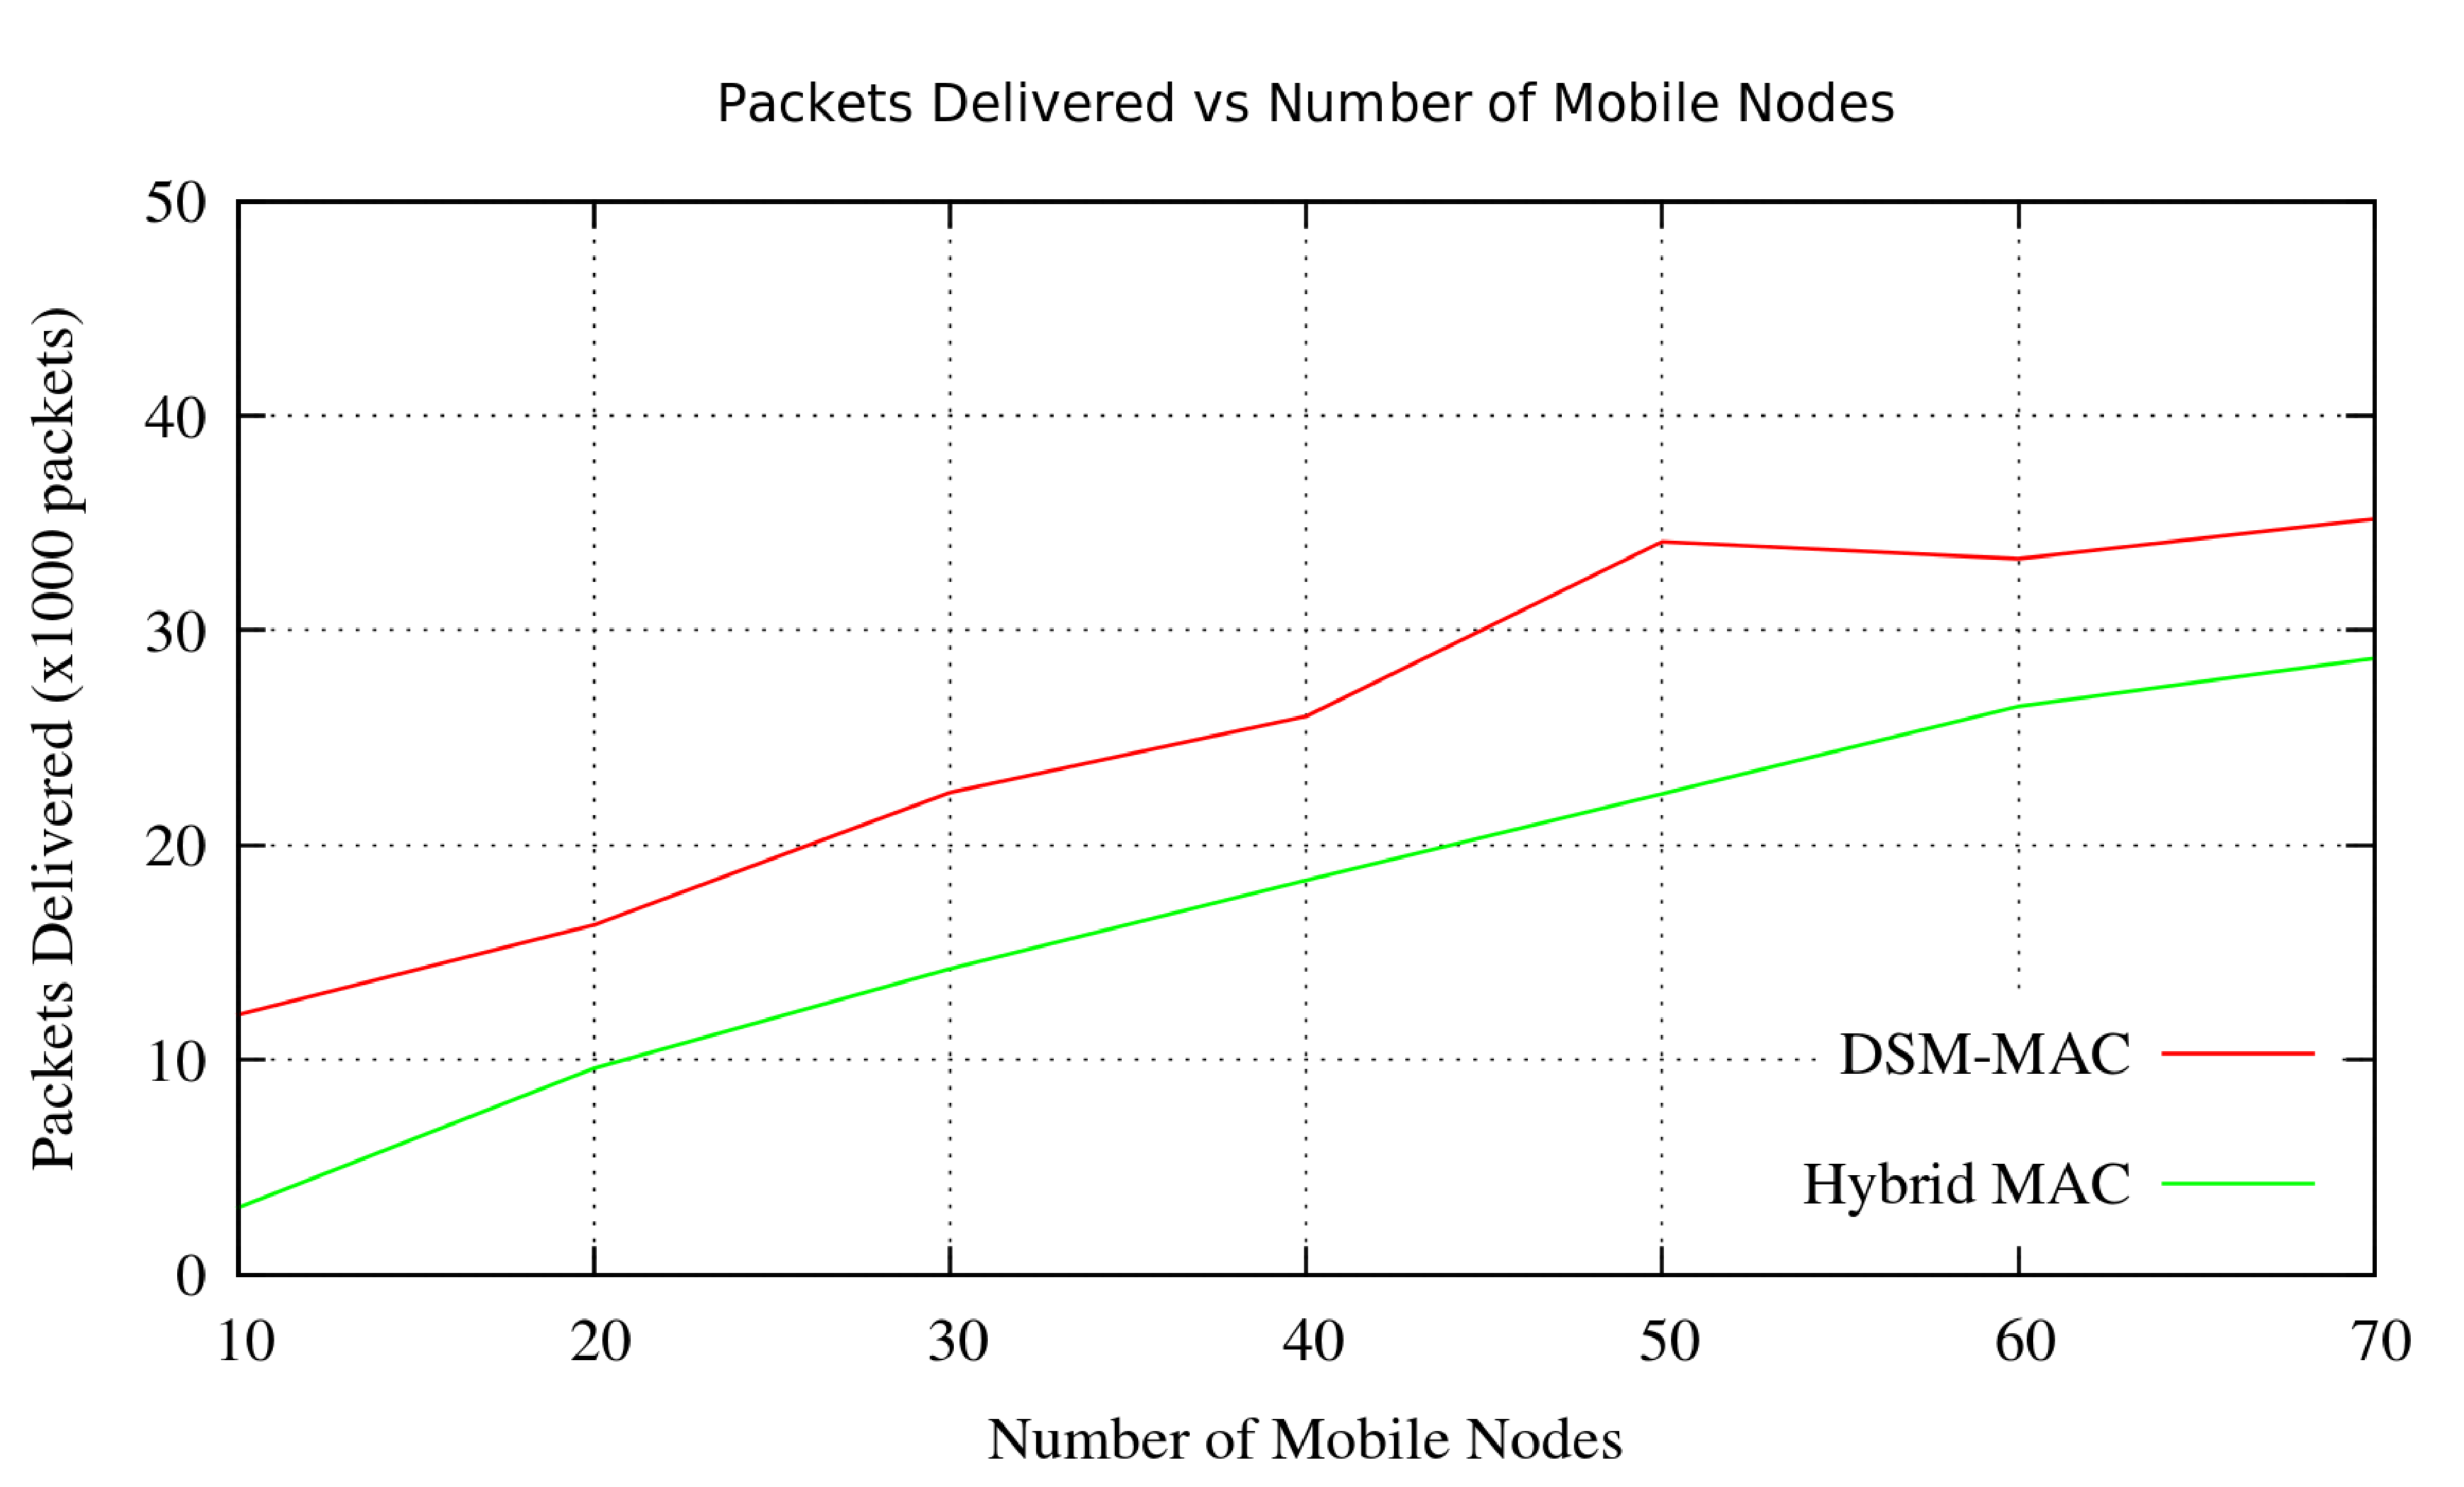
\includegraphics[ width=8.5cm,height=6cm]{pm}
  \end{center}
	\caption{Packets Delivered vs Number of Mobile Nodes}
		\label{fig:pm}
\end{figure}

\begin{figure}[h]{} 
  \begin{center}
		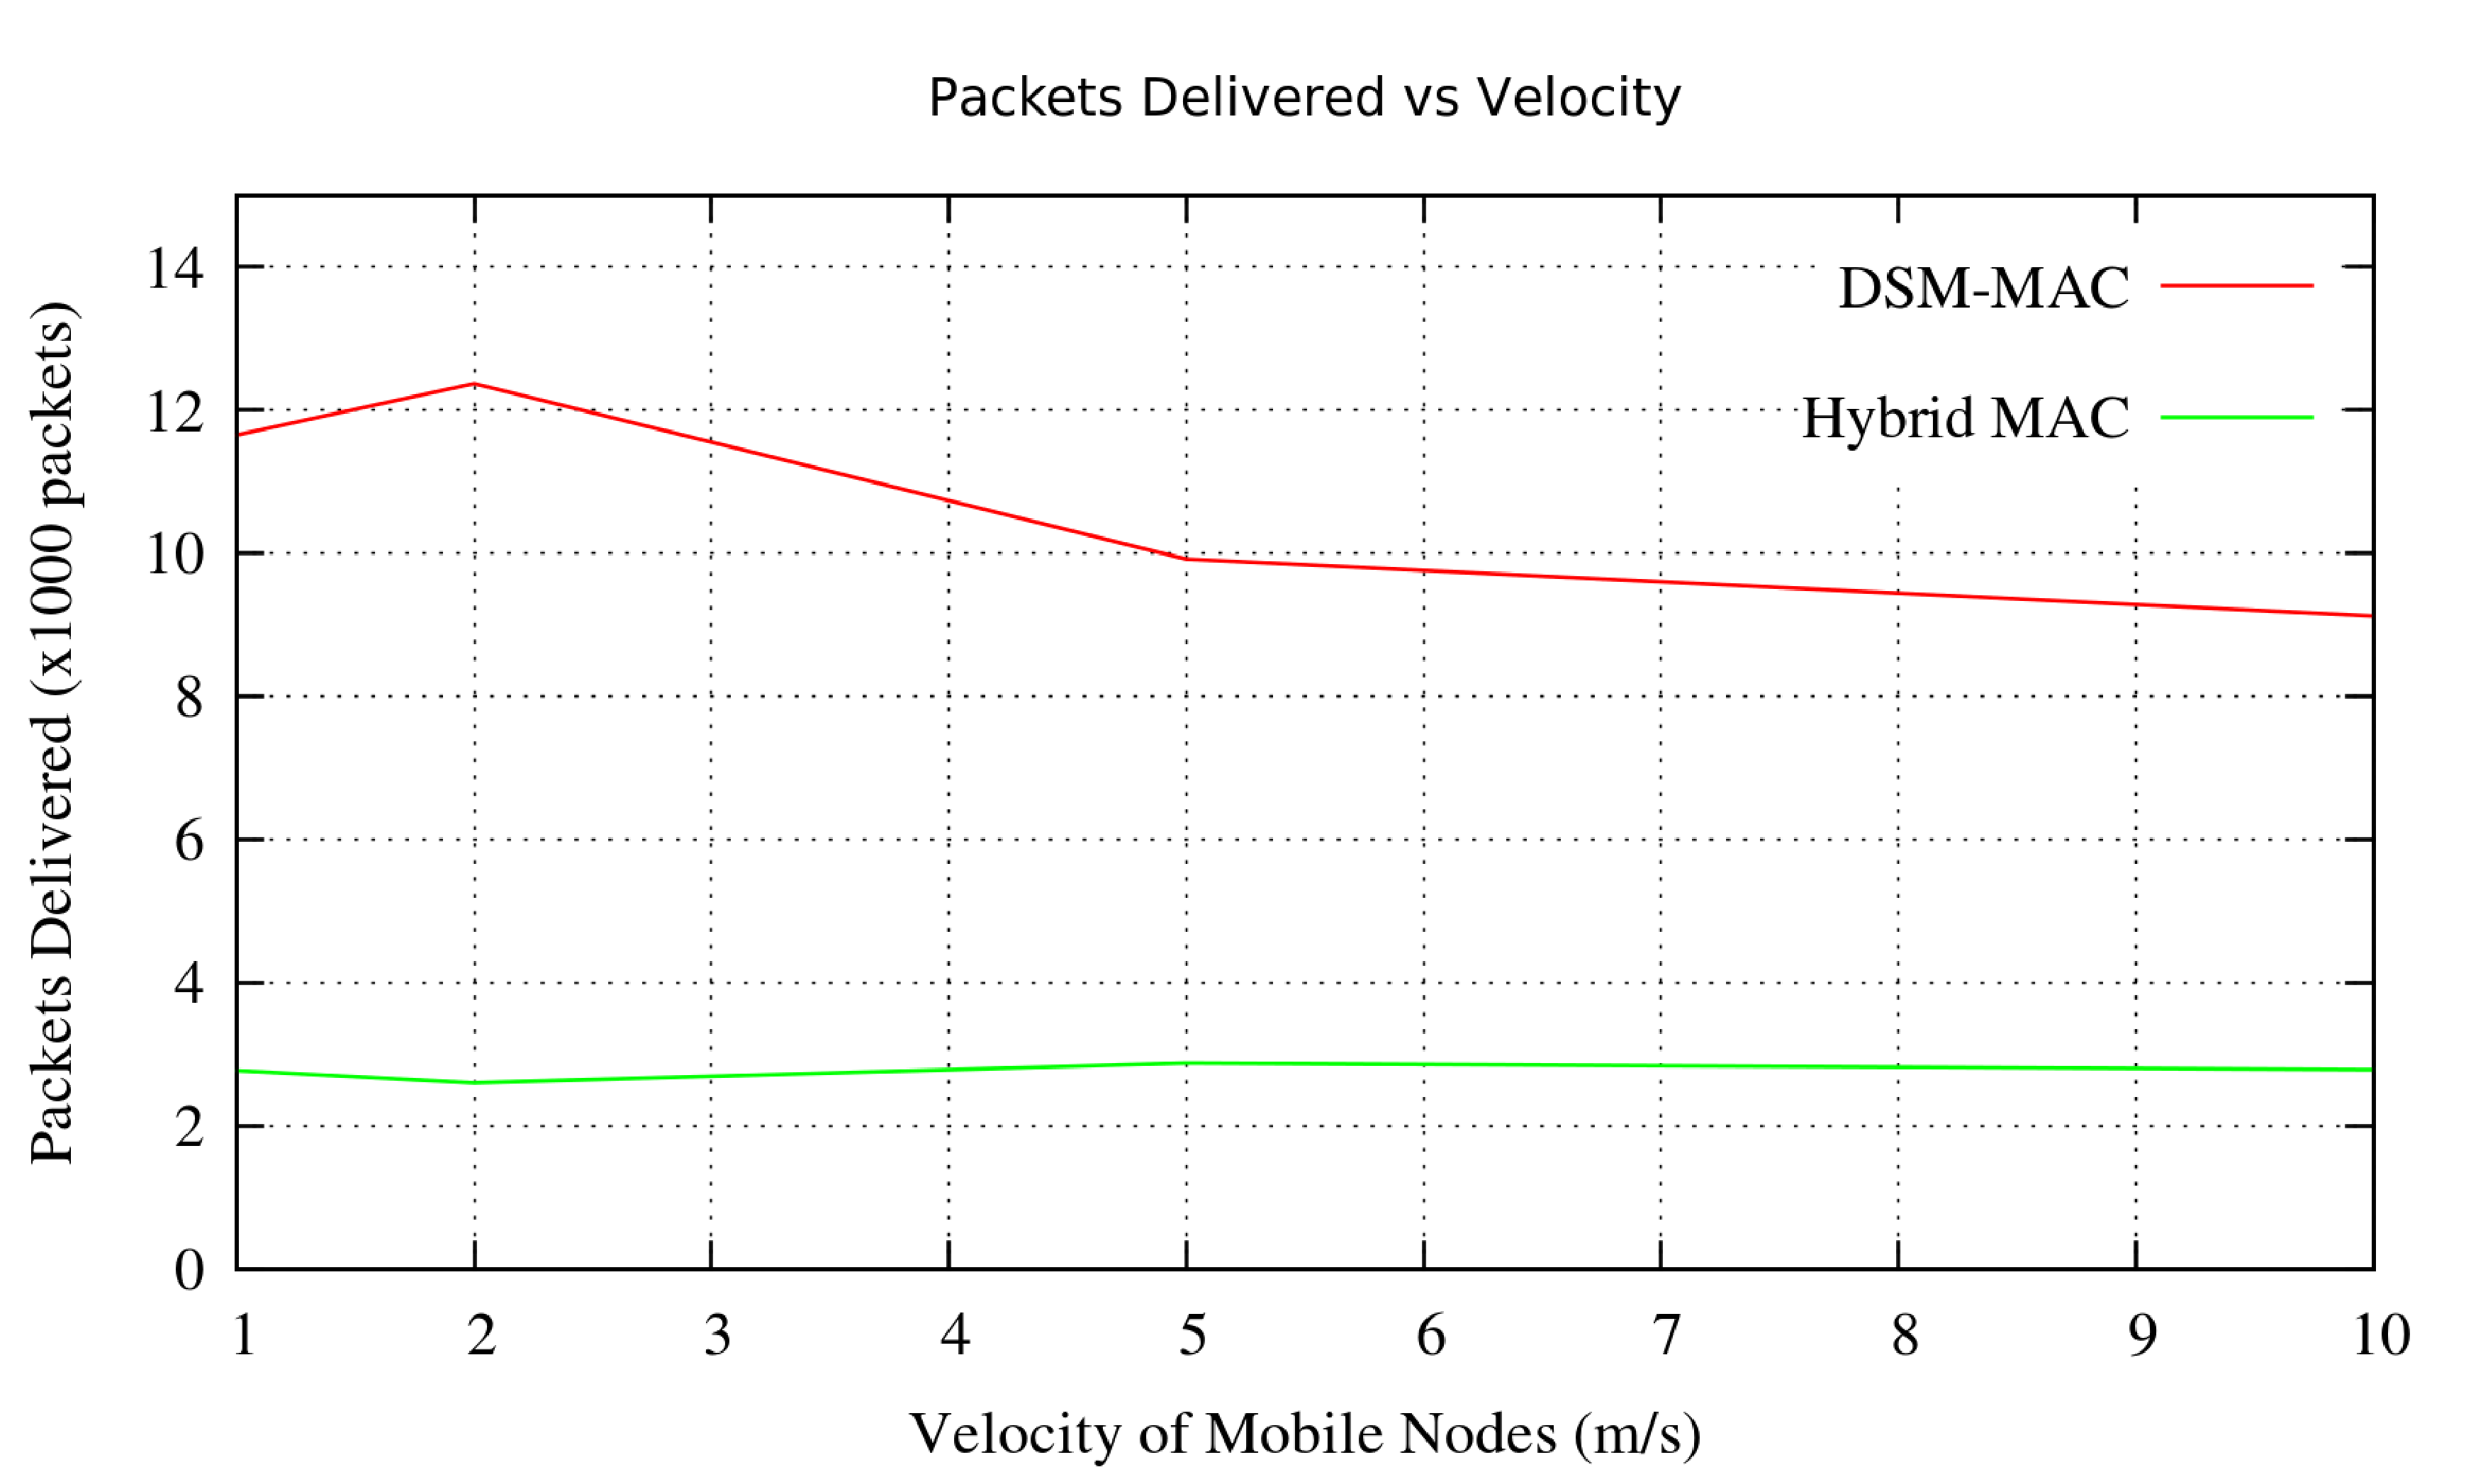
\includegraphics[ width=8.5cm,height=6cm]{pv}
  \end{center}
	\caption{Packets Delivered vs Velocity}
		\label{fig:pv}
\end{figure}
 
\begin{figure}[h]{} 
  \begin{center}
		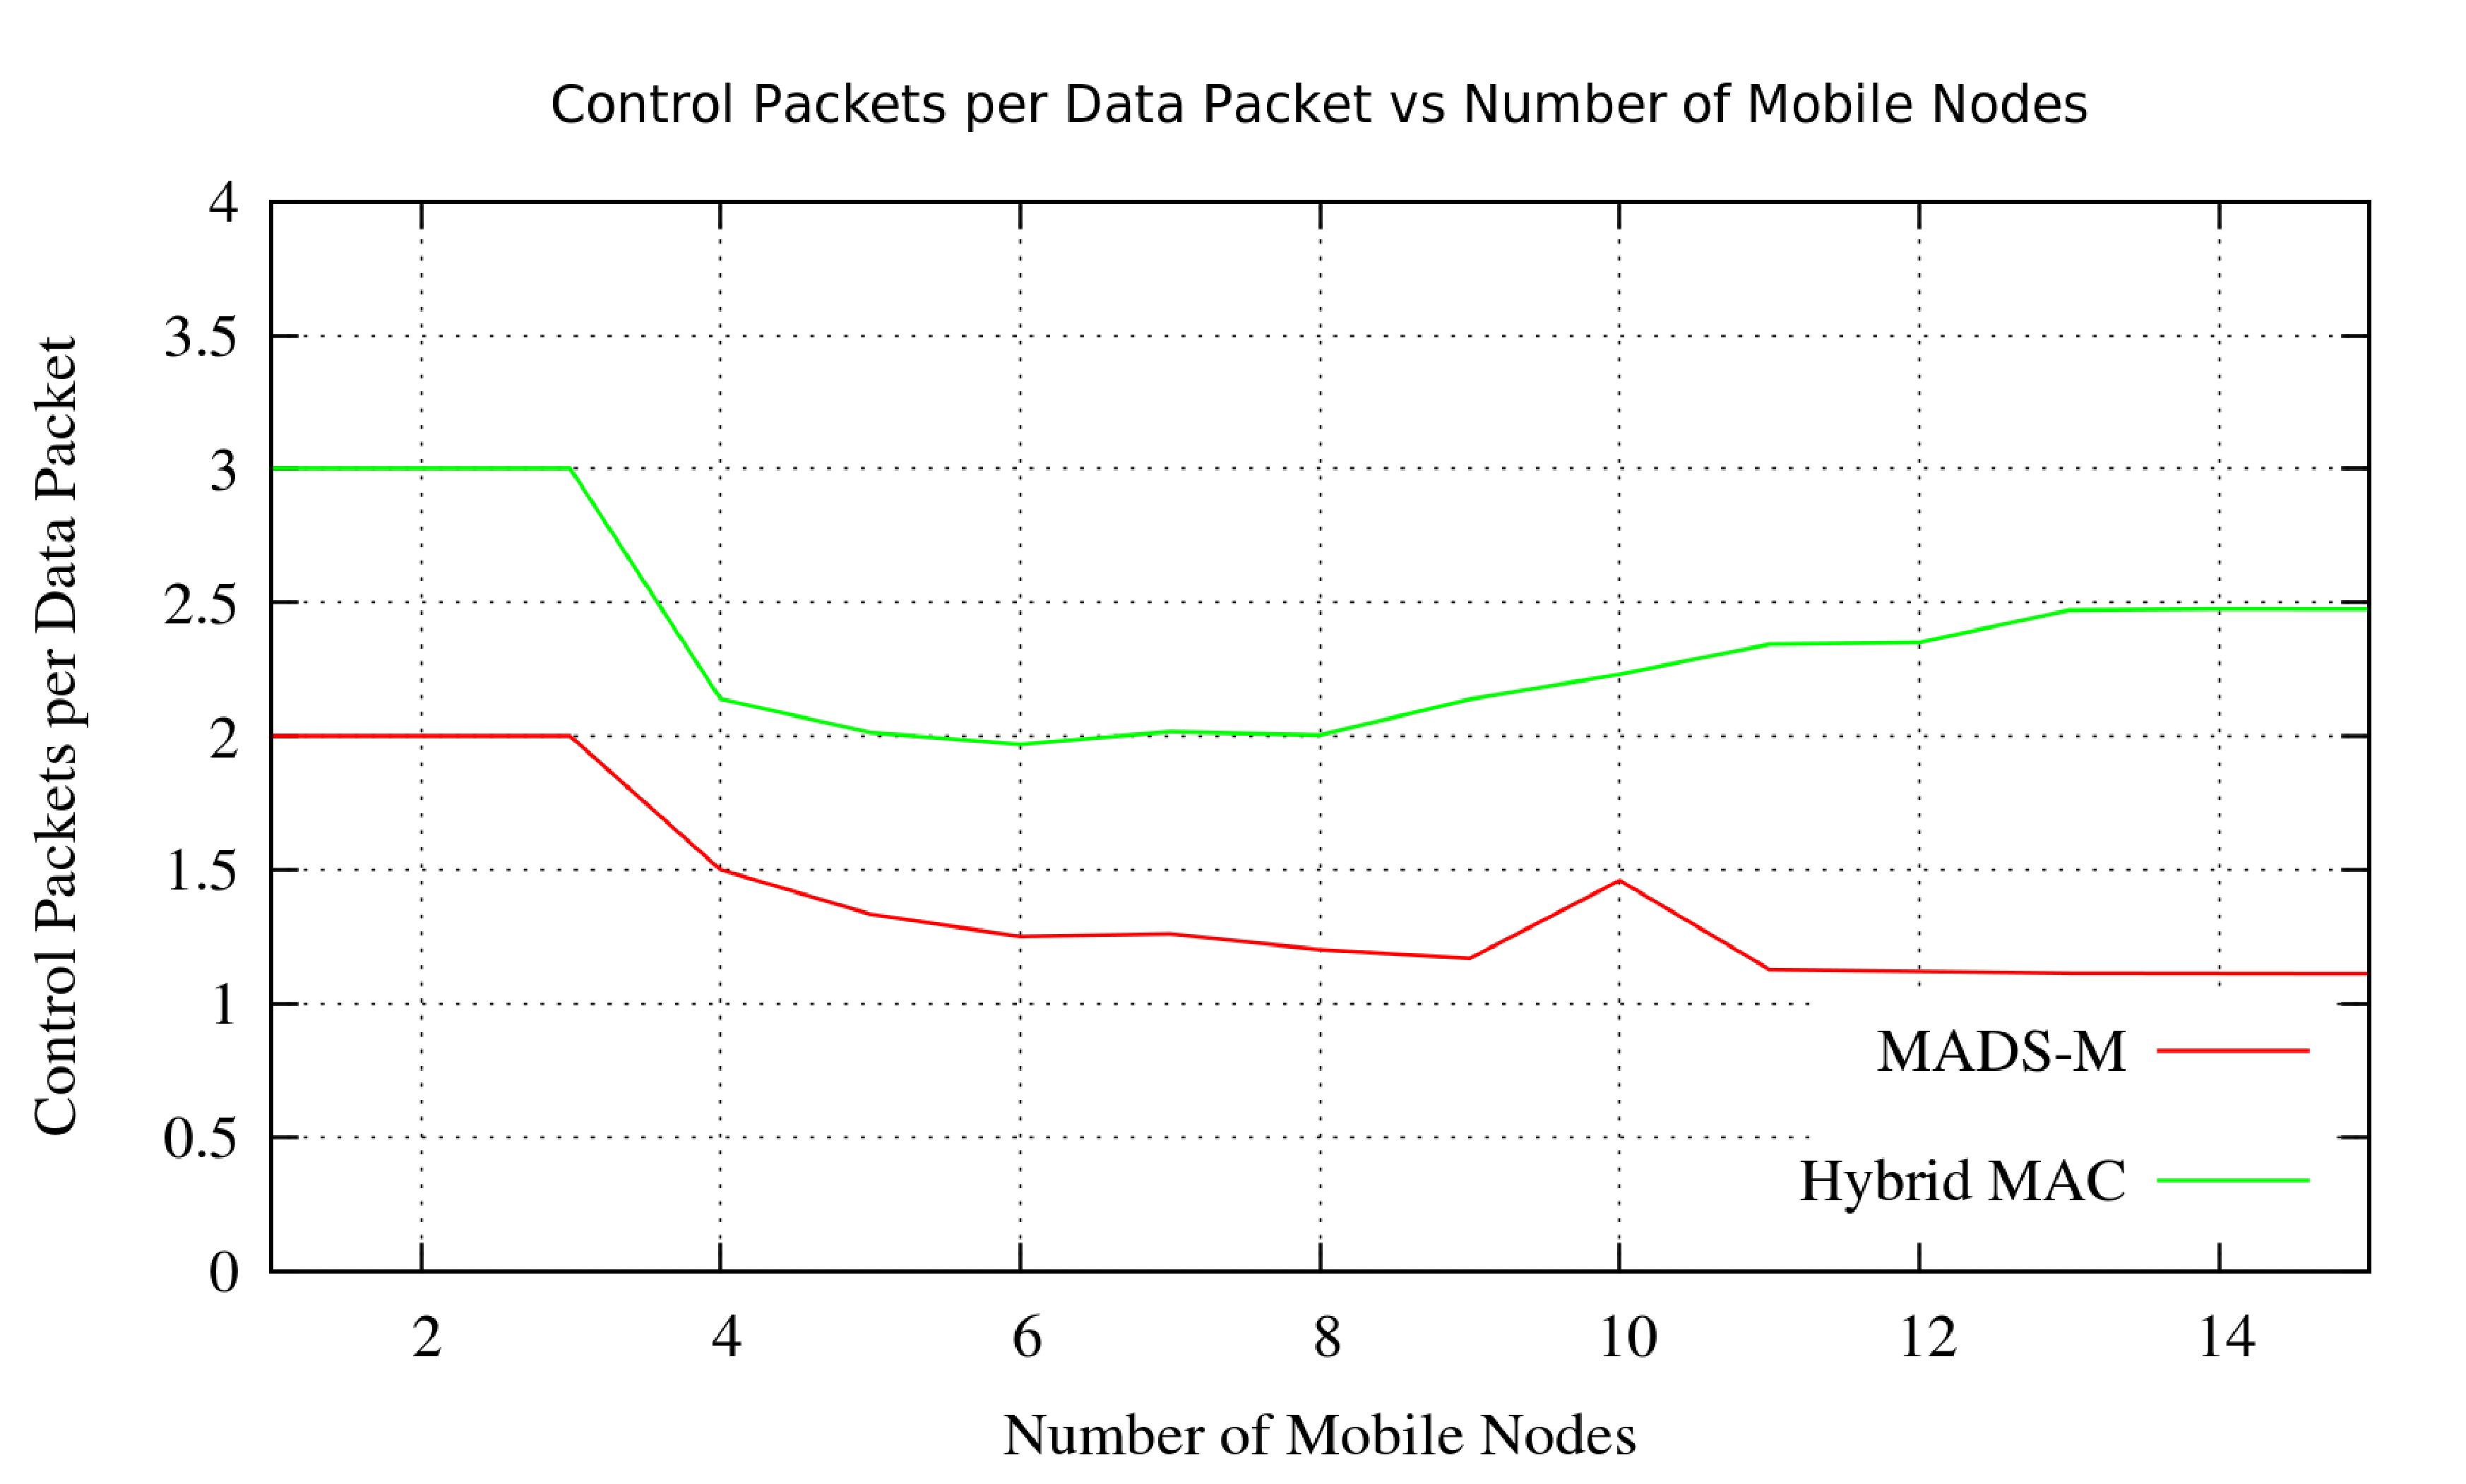
\includegraphics[ width=8.5cm,height=6cm]{cm}
  \end{center}
	\caption{Control Packets vs Number of Mobile Nodes}
		\label{fig:cm}
\end{figure}


The Communication overhead of the proposed protocol is compared with Hybrid MAC and is shown in the Figure \ref{fig:cm}. In this paper, we refer the communciation overhead to the number of control packets used for data communciation. The communication overhead is an essential factor affecting the overall network energy and the amount of channel interference in a network.  In WSN, more energy is spent on communication. If the communication overhead is high, then the overall energy spent for communication is also high. Also for single channel based MAC protocols, interference will be higher for higher communication overhead. Hence it is preferable to have a protocol with less communication overhead. Figure  \ref{fig:cm} plots the number of control packets used w.r.t the number of mobile nodes in a low mobility scenario. Simulation is done by changing the number of mobile nodes from $1$ to $15$. It is clear from Figure \ref{fig:cm} that the number of control packets generated in our approach is lower than that of Hybrid MAC.\\

In the above section, we have compared our approach with Hybrid MAC and have discussed the results based on packet delivery, packet delivery ratio, power consumption and the number of control packets. Even though our approach offers a slightly lower packet delivery ratio compared to Hybrid MAC, it should be noted that our approach performs better in terms of overall packets delivered, energy efficiency and the control overhead. 


\section{Scope}


\chapter{Conclusion} % Main chapter title

\label{conc} % For referencing the chapter elsewhere, use \ref{Chapter1} 

\lhead{Conclusion} % This is for the header on each page - perhaps a shortened title

%----------------------------------------------------------------------------------------

Corrrrrraaaaaaaal.. Write how your protocol performed better and stuff/thangs like dat..


%----------------------------------------------------------------------------------------
%	THESIS CONTENT - APPENDICES
%----------------------------------------------------------------------------------------

\addtocontents{toc}{\vspace{2em}} % Add a gap in the Contents, for aesthetics

\appendix % Cue to tell LaTeX that the following 'chapters' are Appendices

% Include the appendices of the thesis as separate files from the Appendices folder
% Uncomment the lines as you write the Appendices

% Appendix A

\chapter{Appendix Title Here} % Main appendix title

\label{AppendixA} % For referencing this appendix elsewhere, use \ref{AppendixA}

\lhead{Appendix A. \emph{Appendix Title Here}} % This is for the header on each page - perhaps a shortened title

Write your Appendix content here.
%\input{Appendices/AppendixB}
%\input{Appendices/AppendixC}

\addtocontents{toc}{\vspace{2em}} % Add a gap in the Contents, for aesthetics

\backmatter

%----------------------------------------------------------------------------------------
%	BIBLIOGRAPHY
%----------------------------------------------------------------------------------------

\label{Bibliography}

\lhead{\emph{Bibliography}} % Change the page header to say "Bibliography"

\bibliographystyle{unsrtnat} % Use the "unsrtnat" BibTeX style for formatting the Bibliography

\bibliography{Bibliography} % The references (bibliography) information are stored in the file named "Bibliography.bib"

\end{document}  
